\documentclass[aspectratio=169,17pt]{beamer}

\usepackage{amsmath}
\usepackage{mathptmx}
\usepackage{helvet}
\usepackage{graphicx}

\definecolor{smitten}{HTML}{CD3487}
\definecolor{corn}{HTML}{FFF265}
\definecolor{midnightgreen}{HTML}{004850}
\definecolor{stpatricksblue}{HTML}{1F2882}
\definecolor{independence}{HTML}{354261}
\definecolor{spanishgrey}{HTML}{989C94}
\definecolor{cafeaulait}{HTML}{A57548}

\beamertemplatenavigationsymbolsempty
\setbeamertemplate{itemize item}{\textbullet}
\setbeamertemplate{blocks}[rounded][shadow=false]
\usecolortheme{seagull}
\usefonttheme[stillsansseriflarge]{serif}
\setbeamercolor{frametitle}{bg=white, fg=independence}
\setbeamercolor{title}{bg=yellow,fg=smitten}
\setbeamercolor{author}{bg=yellow,fg=smitten}
\setbeamercolor{text}{bg=white, bg=black}
\setbeamercolor{background canvas}{bg=cafeaulait}
\setbeamercolor{block title}{bg=white,fg=independence}
\setbeamercolor{block body}{bg=white,fg=black}

\title{\textbf{Solving Logarithmic and Exponential Equations}}
\subtitle{Quick Start}
\author{\textsf{\textbf{Success in College Math}}}
\date{}

\begin{document}

\begin{frame}
	\titlepage
\end{frame}

\begin{frame}
	\frametitle{Overview}
	\begin{block}{This video will cover:} \pause
	\begin{enumerate}
		\item Inverse Properties of Logarithms and Exponential Functions \pause
		\item Solving Exponential Equations \pause
		\item Solving Logarithmic Equations
	\end{enumerate}
	\end{block}
\end{frame}

\begin{frame}
	\frametitle{Inverse Properties of Logarithms and Exponential Functions}
	\begin{columns}
		\column{0.5\textwidth}
		
		\begin{block}{}
		For all $x$,
		$$\log_b{b^x} = x.$$
		\end{block}
		
		\column{0.5\textwidth}
		
		\begin{block}{}
		For $x > 0$,
		$$b^{log_b{x}} = x.$$
		\end{block}
	
	\end{columns}
\end{frame}

\begin{frame}
	\frametitle{How To - Solve Exponential Equations}
	To solve an equation containing an exponential expression: \pause
	\begin{enumerate}
		\item Isolate the exponential expression. \pause
		\item Take the logarithm of both sides. Use the same base for the logarithm as the exponential expression. \pause
		\item Cancel the logarithm and exponential expression using the Inverse Property. \pause
		\item Solve the resulting equation.
	\end{enumerate}
\end{frame}

\begin{frame}[t]
	\frametitle{Example 1}
	Solve the equation. Round your answer to three decimal places where appropriate.
	$$4 \cdot 9^{2x} = 14$$
\end{frame}

\begin{frame}
	\frametitle{Example 1}
	\begin{columns}
		\column{0.3\textwidth}
			Solve for the exponential expression.
		\column{0.7\textwidth}
			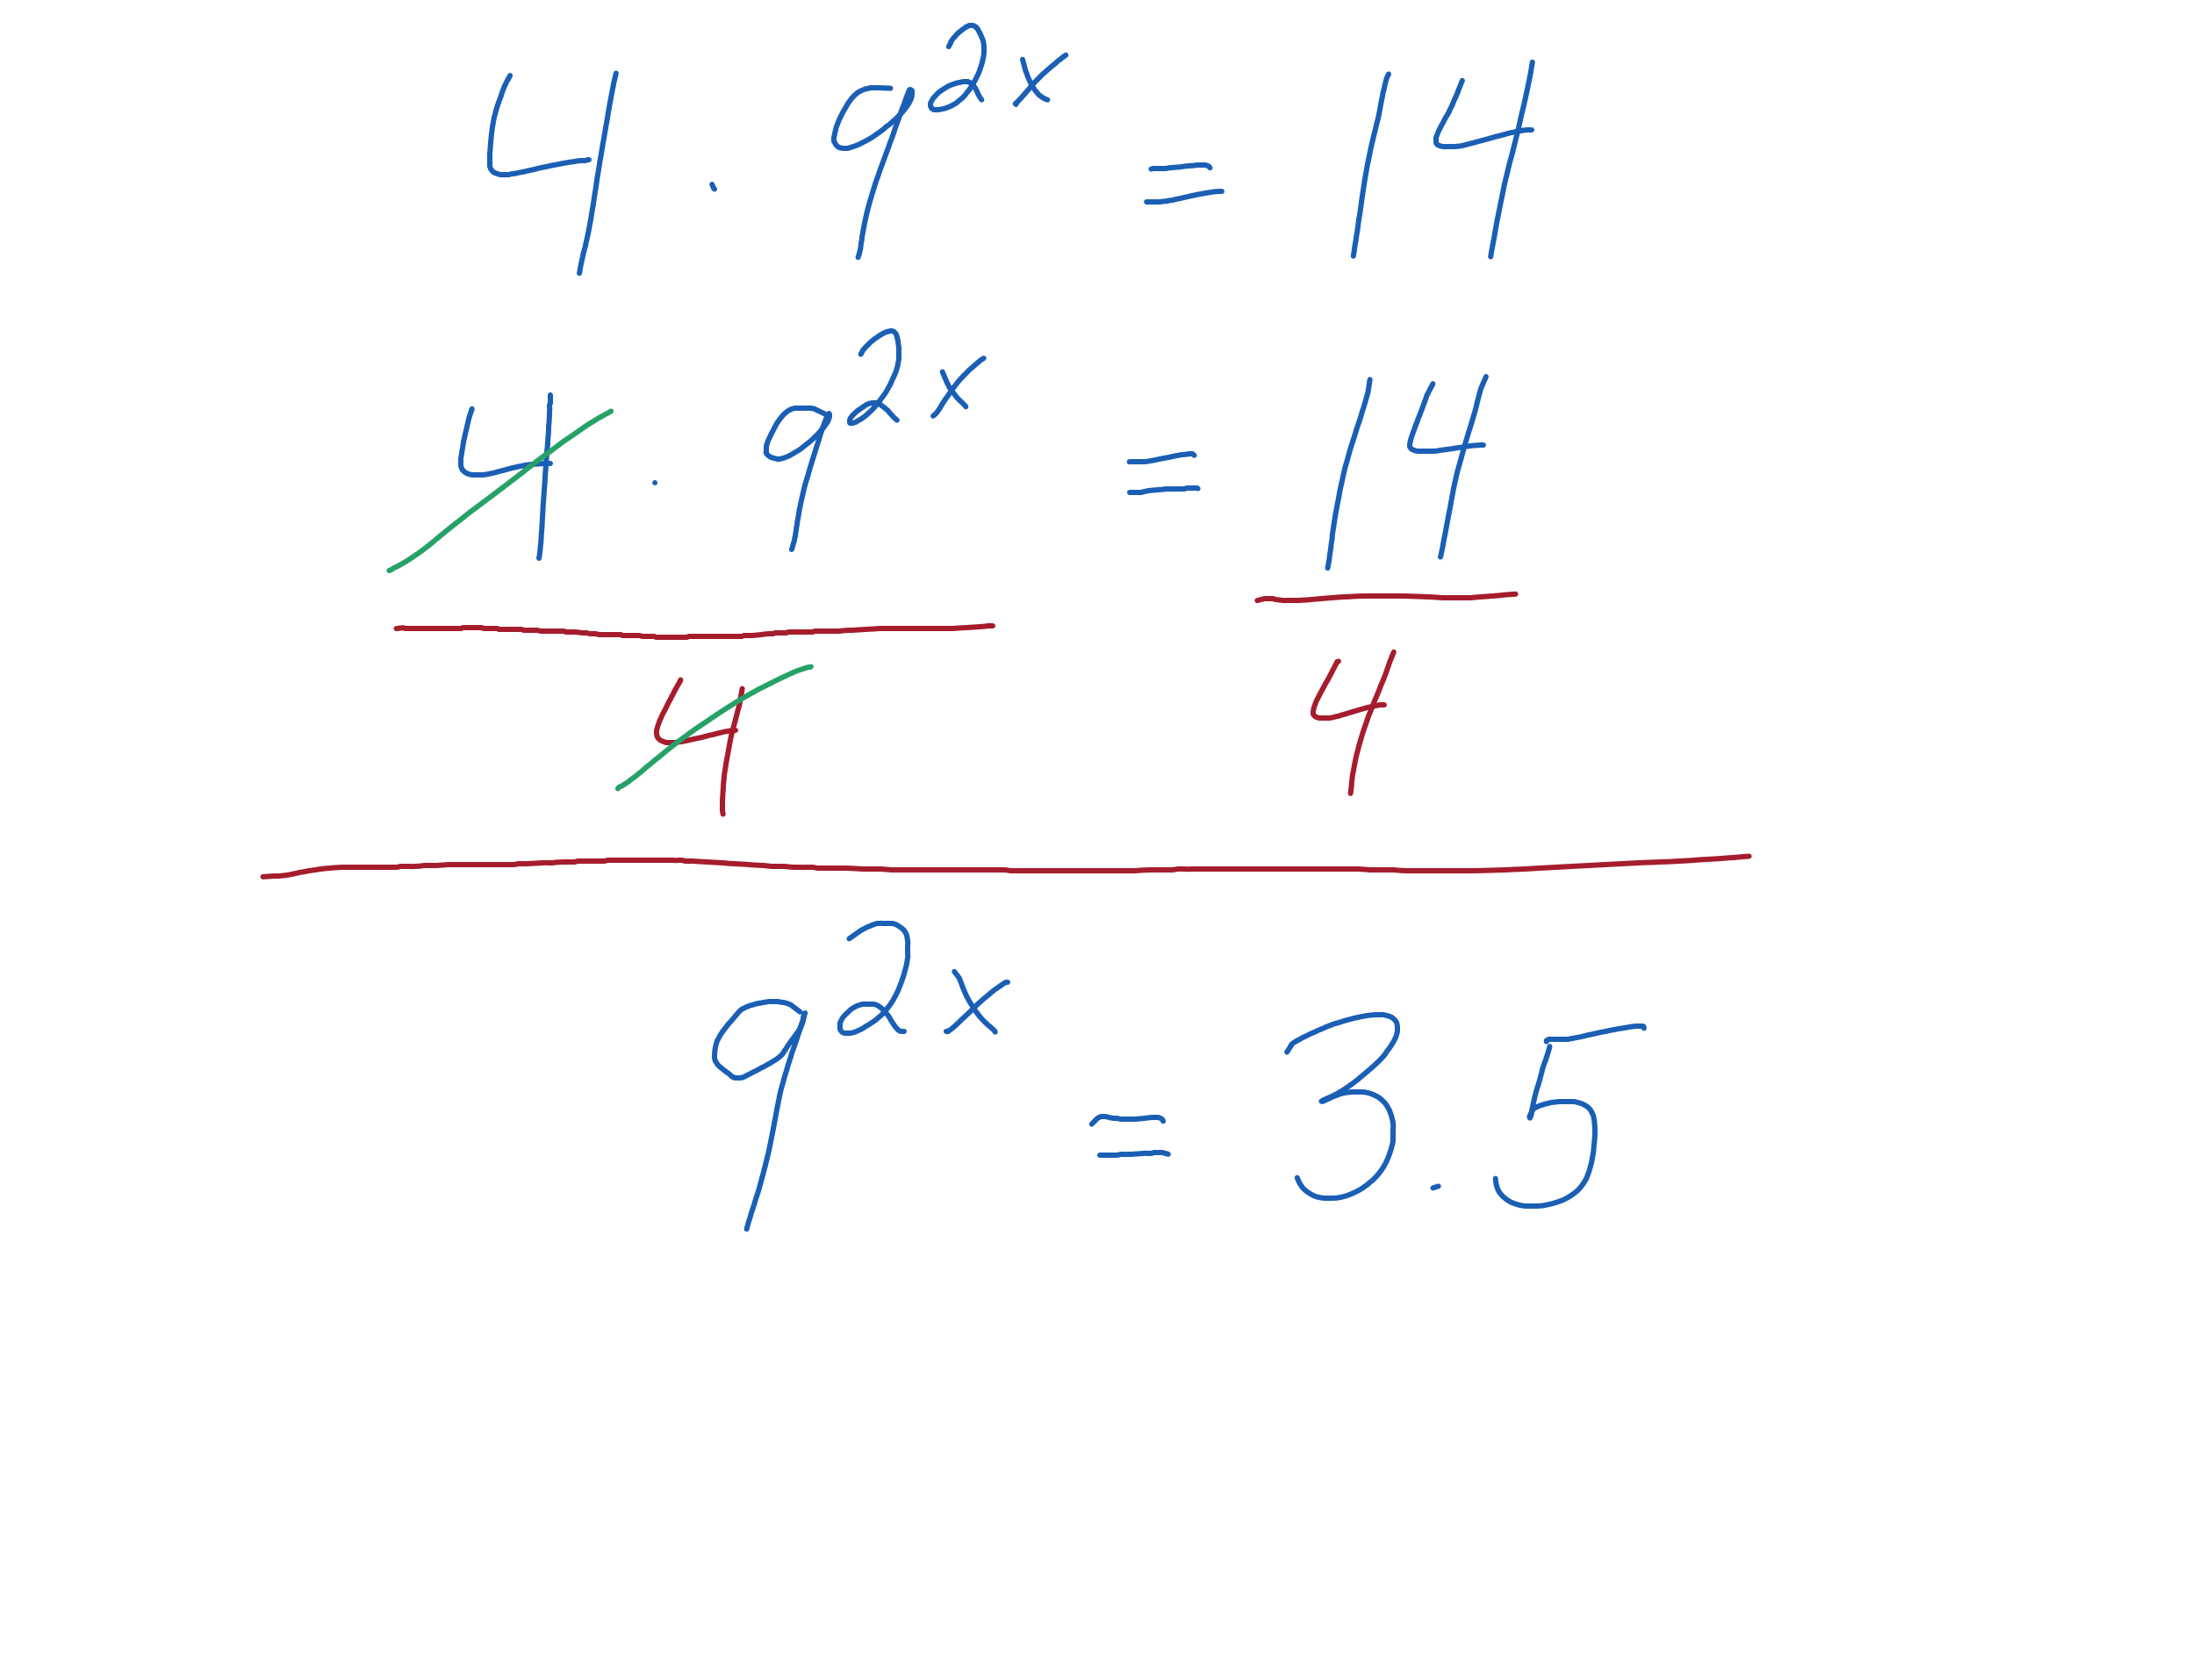
\includegraphics[width=\textwidth]{logarithmic_equations-work_01.png}
	\end{columns}
\end{frame}

\begin{frame}
	\frametitle{Example 1}
	\begin{columns}
		\column{0.3\textwidth}
		\begin{itemize} \small
			\item Take the logarithm base 9 of both sides.
			\item Cancel the logarithm and exponent.
		\end{itemize}
		\column{0.7\textwidth}
			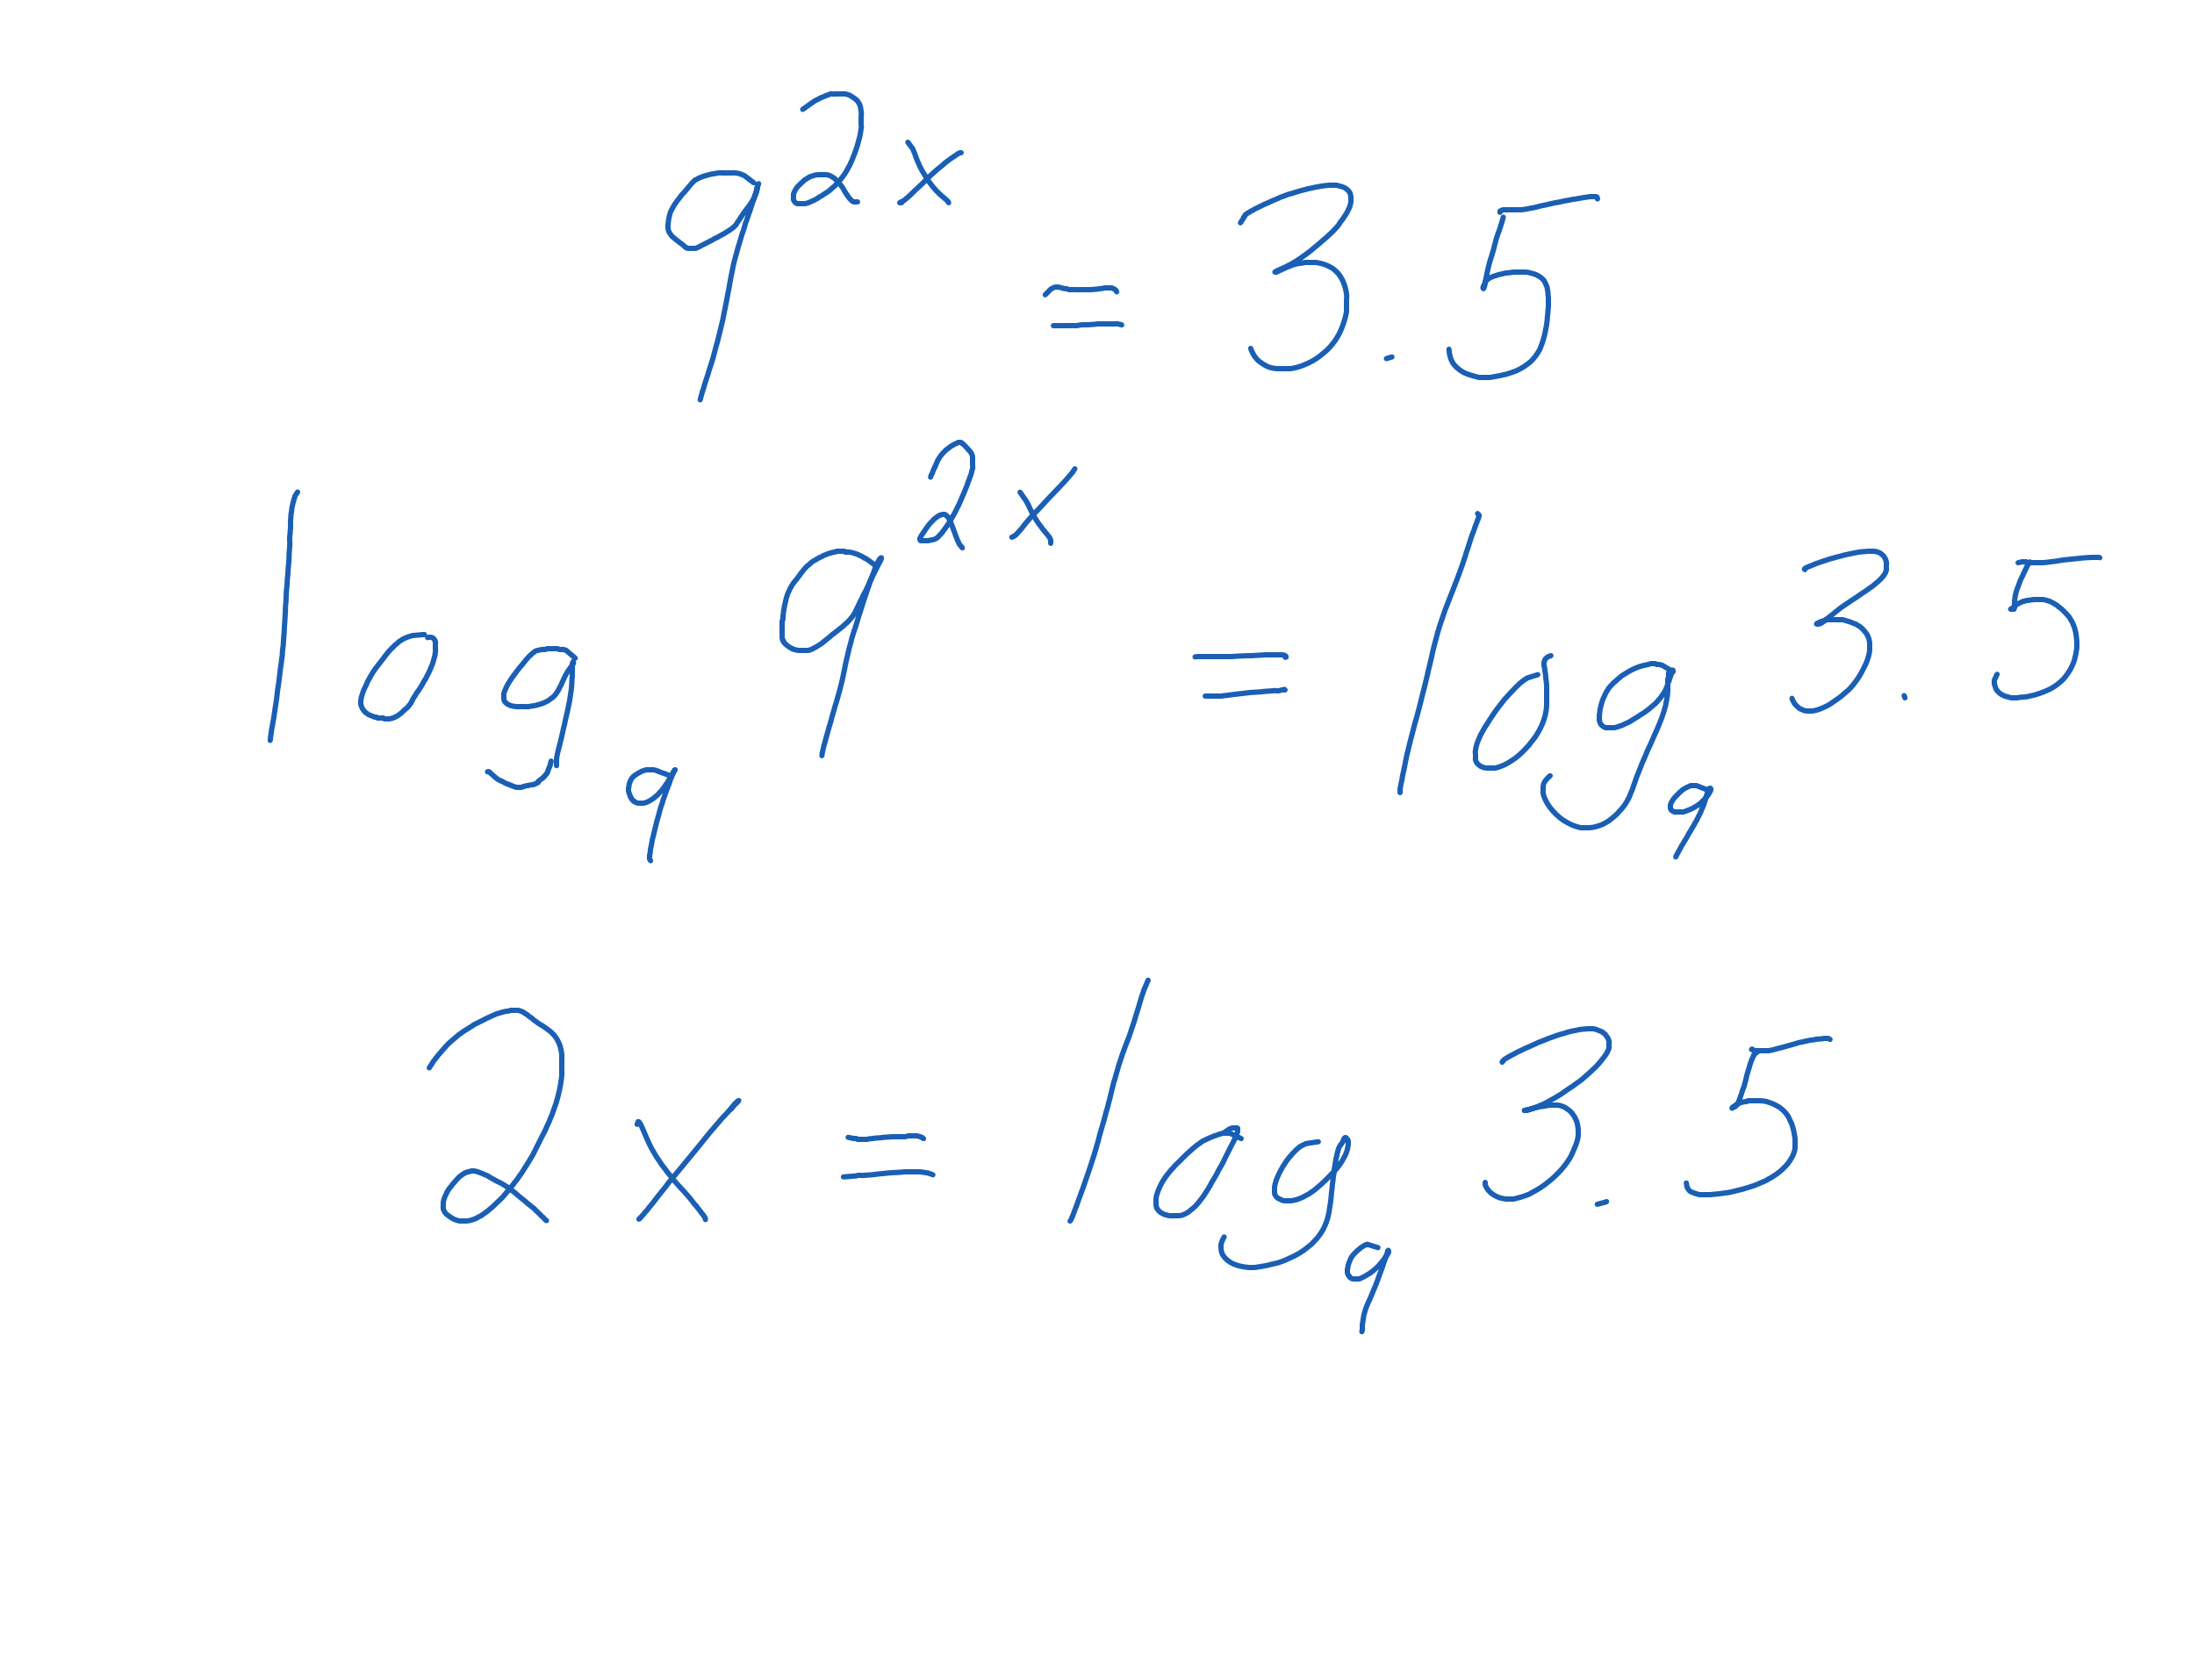
\includegraphics[width=\textwidth]{logarithmic_equations-work_02.png}
	\end{columns}
\end{frame}

\begin{frame}
	\frametitle{Example 1}
	\begin{columns}
		\column{0.3\textwidth}
		\begin{itemize} \small
			\item Solve for $x$. \vspace{\fill}
			\item Round your answer to three decimal places.
		\end{itemize}
		\column{0.7\textwidth}
			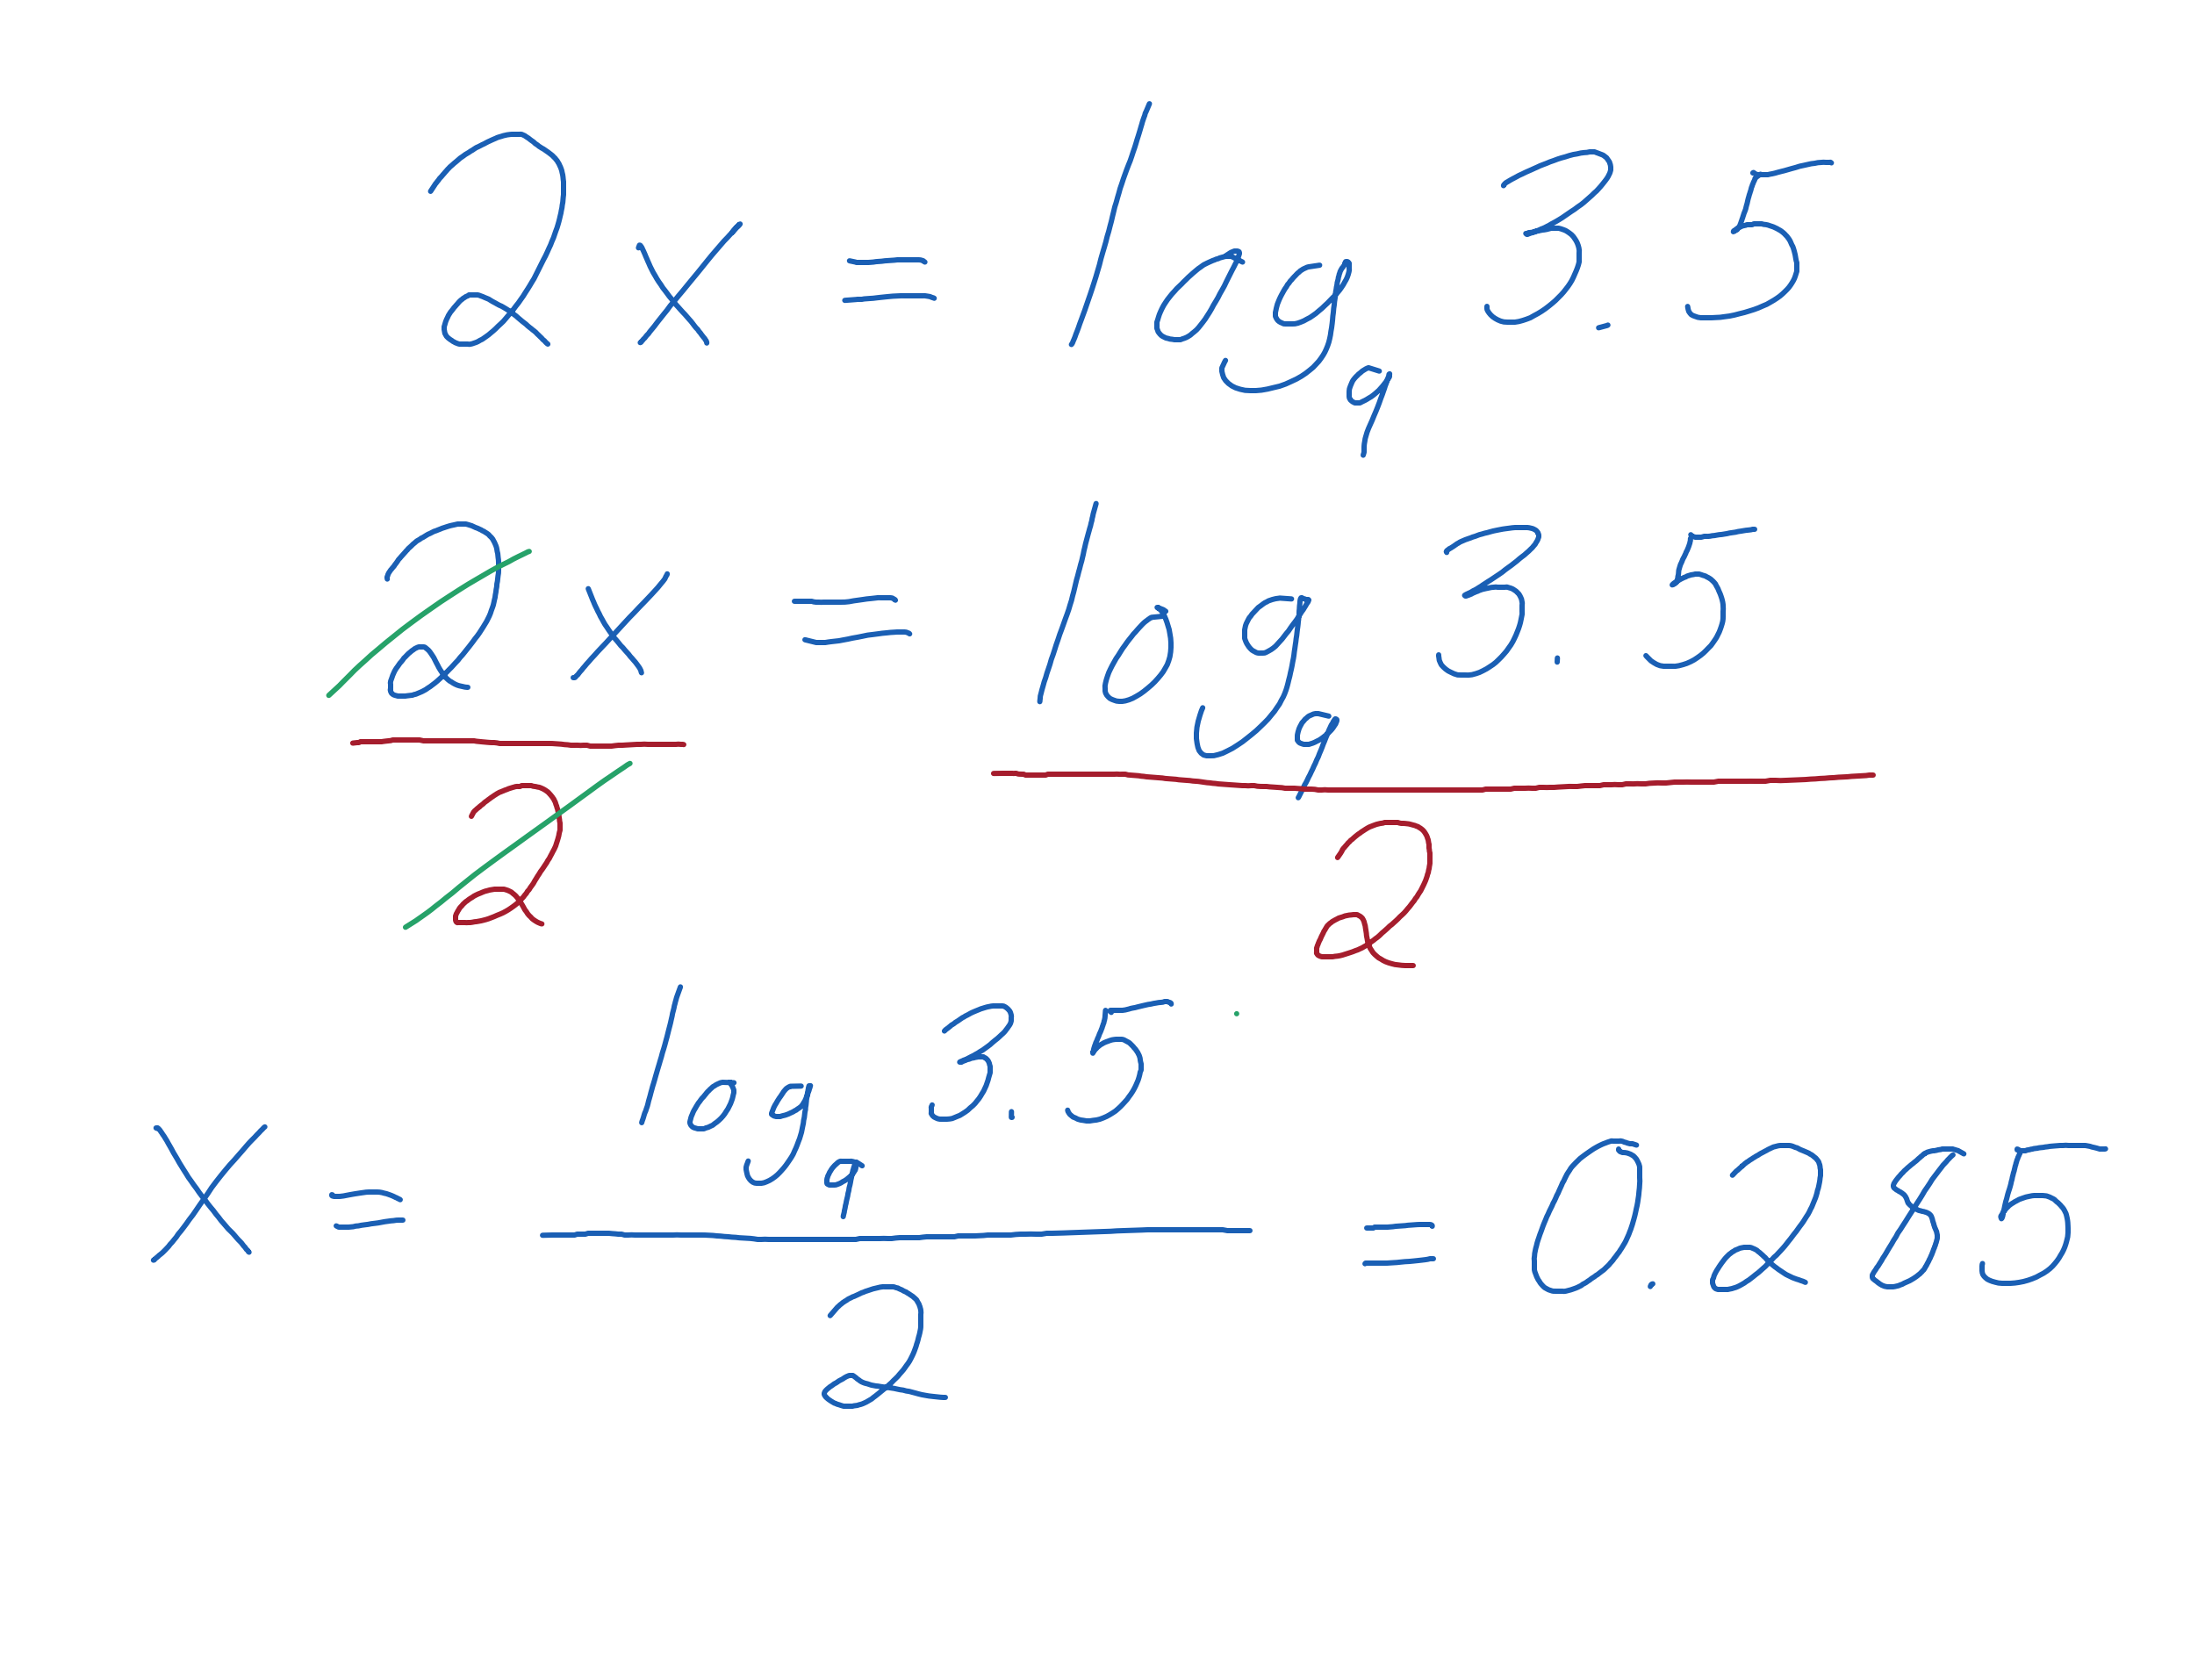
\includegraphics[width=\textwidth]{logarithmic_equations-work_03.png}
	\end{columns}
\end{frame}

\begin{frame}
	\frametitle{Example 1}
	\begin{columns}
		\column{0.3\textwidth}
		\begin{itemize} \small
			\item Solve for $x$. \vspace{\fill}
			\item Round your answer to three decimal places.
		\end{itemize}
		\column{0.7\textwidth}
			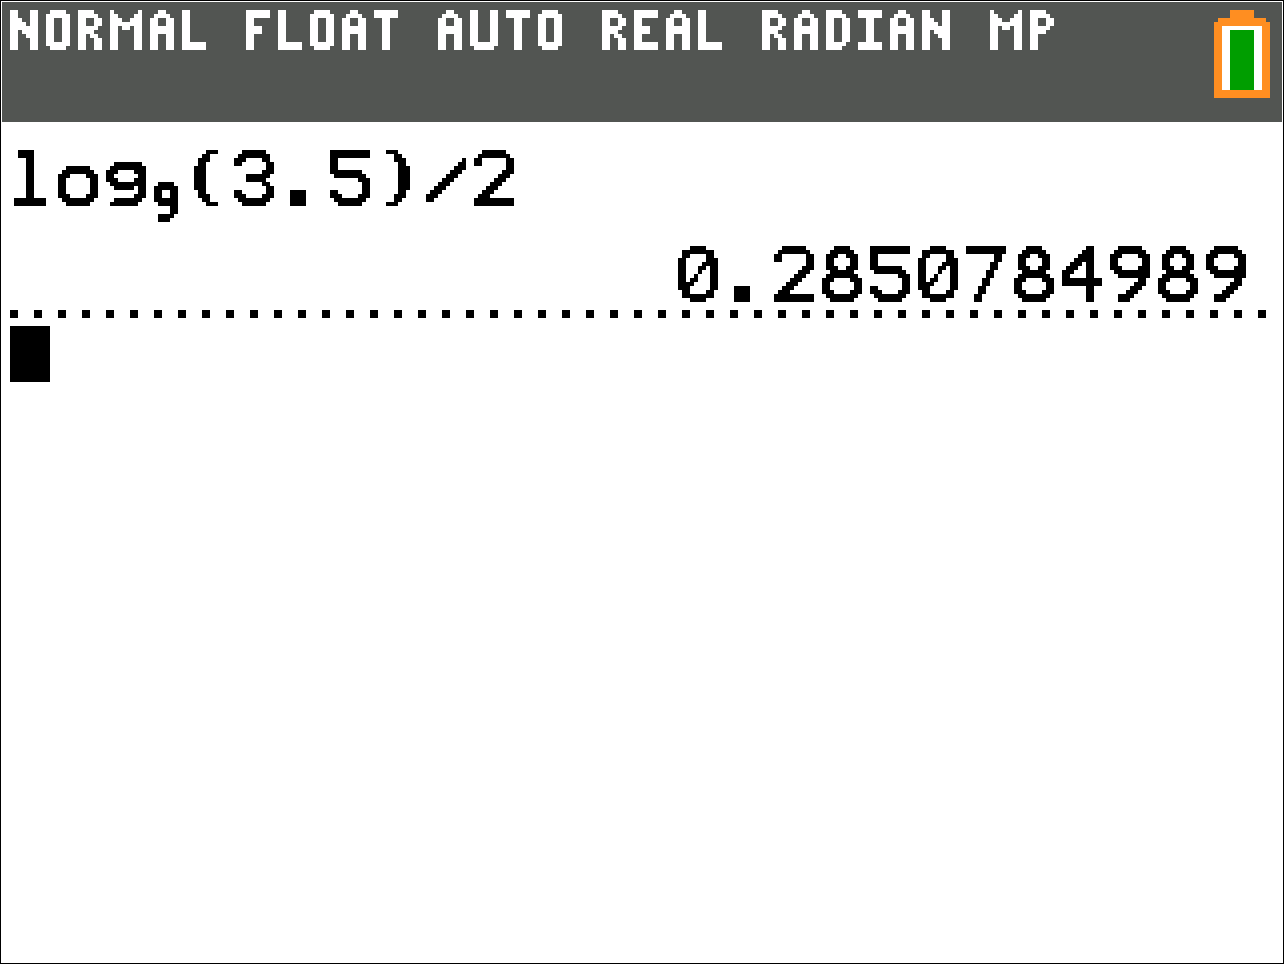
\includegraphics[width=\textwidth]{Capture 1.png}
	\end{columns}
\end{frame}

\begin{frame}[t]
	\frametitle{Example 2}
	Solve the equation. Round your answer to three decimal places where appropriate.
	$$10^{2x-18} + 12 = -3$$
\end{frame}

\begin{frame}
	\frametitle{Example 2}
	\begin{columns}
		\column{0.3\textwidth}
			Solve for the exponential expression.
		\column{0.7\textwidth}
			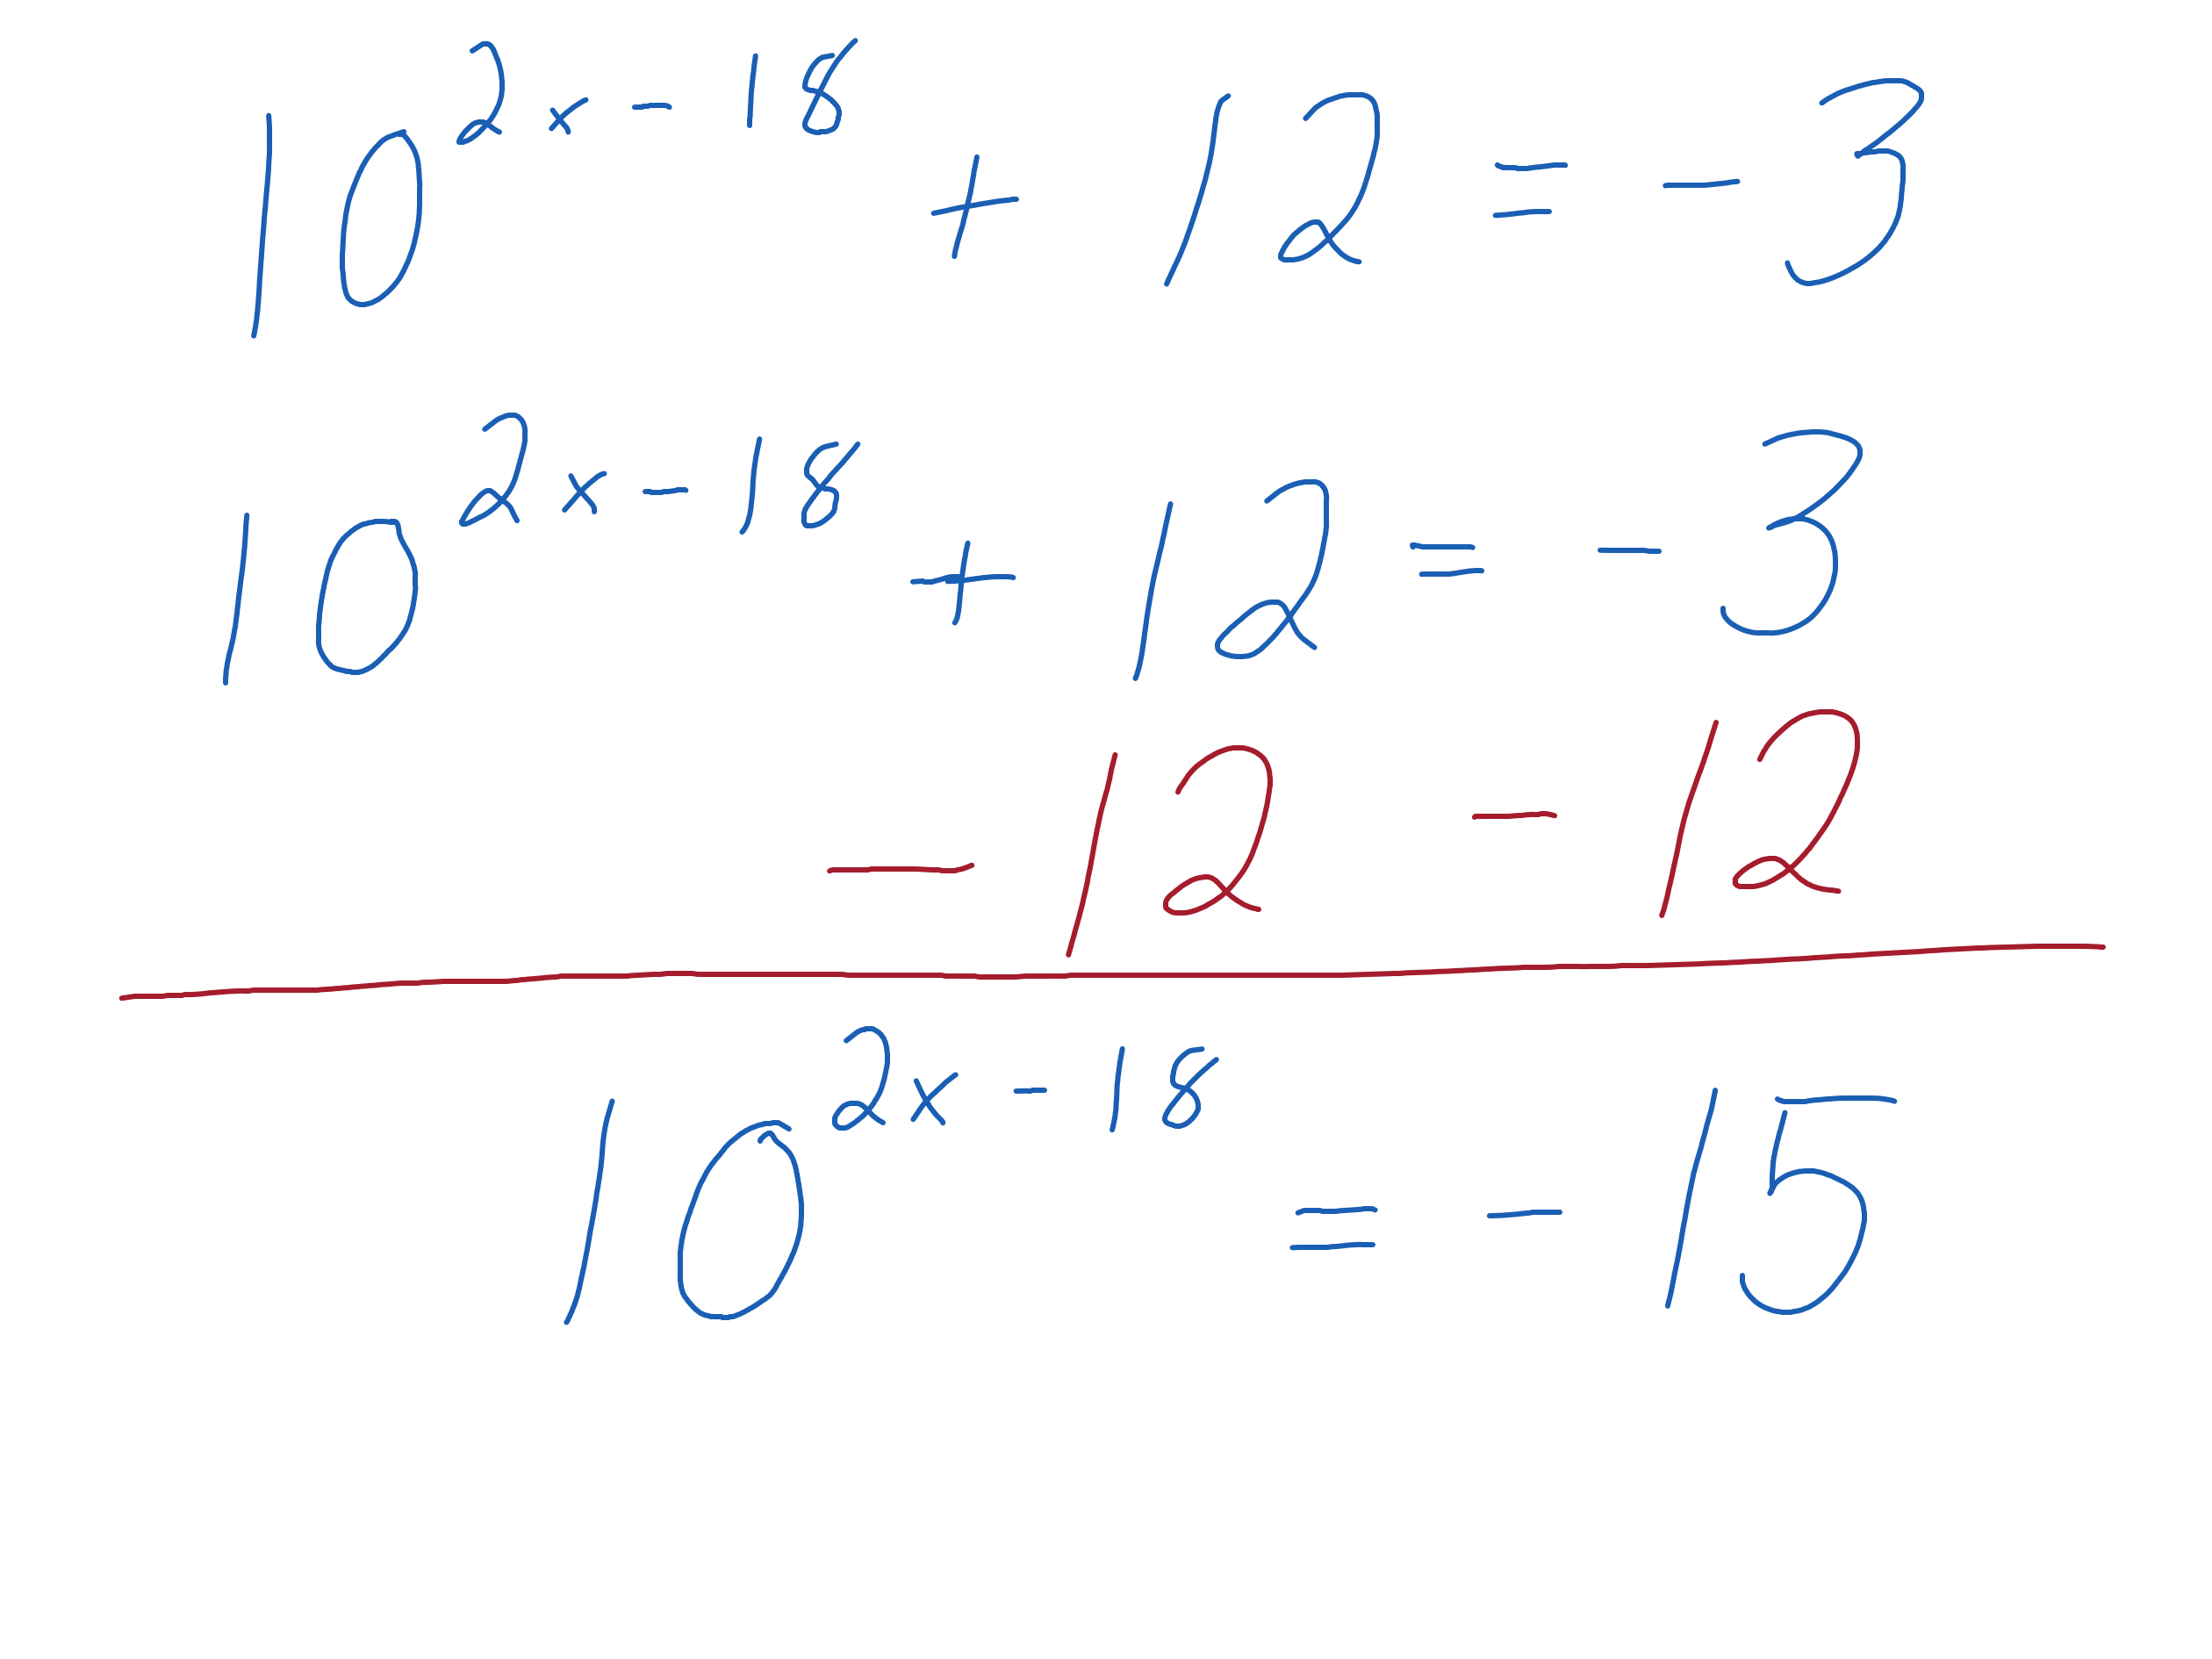
\includegraphics[width=\textwidth]{logarithmic_equations-work_04.png}
	\end{columns}
\end{frame}

\begin{frame}
	\frametitle{Example 2}
	\begin{columns}
		\column{0.3\textwidth}
		\begin{itemize} \small
			\item Take the common logarithm of both sides. \vspace{\fill}
			\item The common logarithm isn't defined for $-15$, 
			so the equation does not have (real number) solutions.
		\end{itemize}
		\column{0.7\textwidth}
			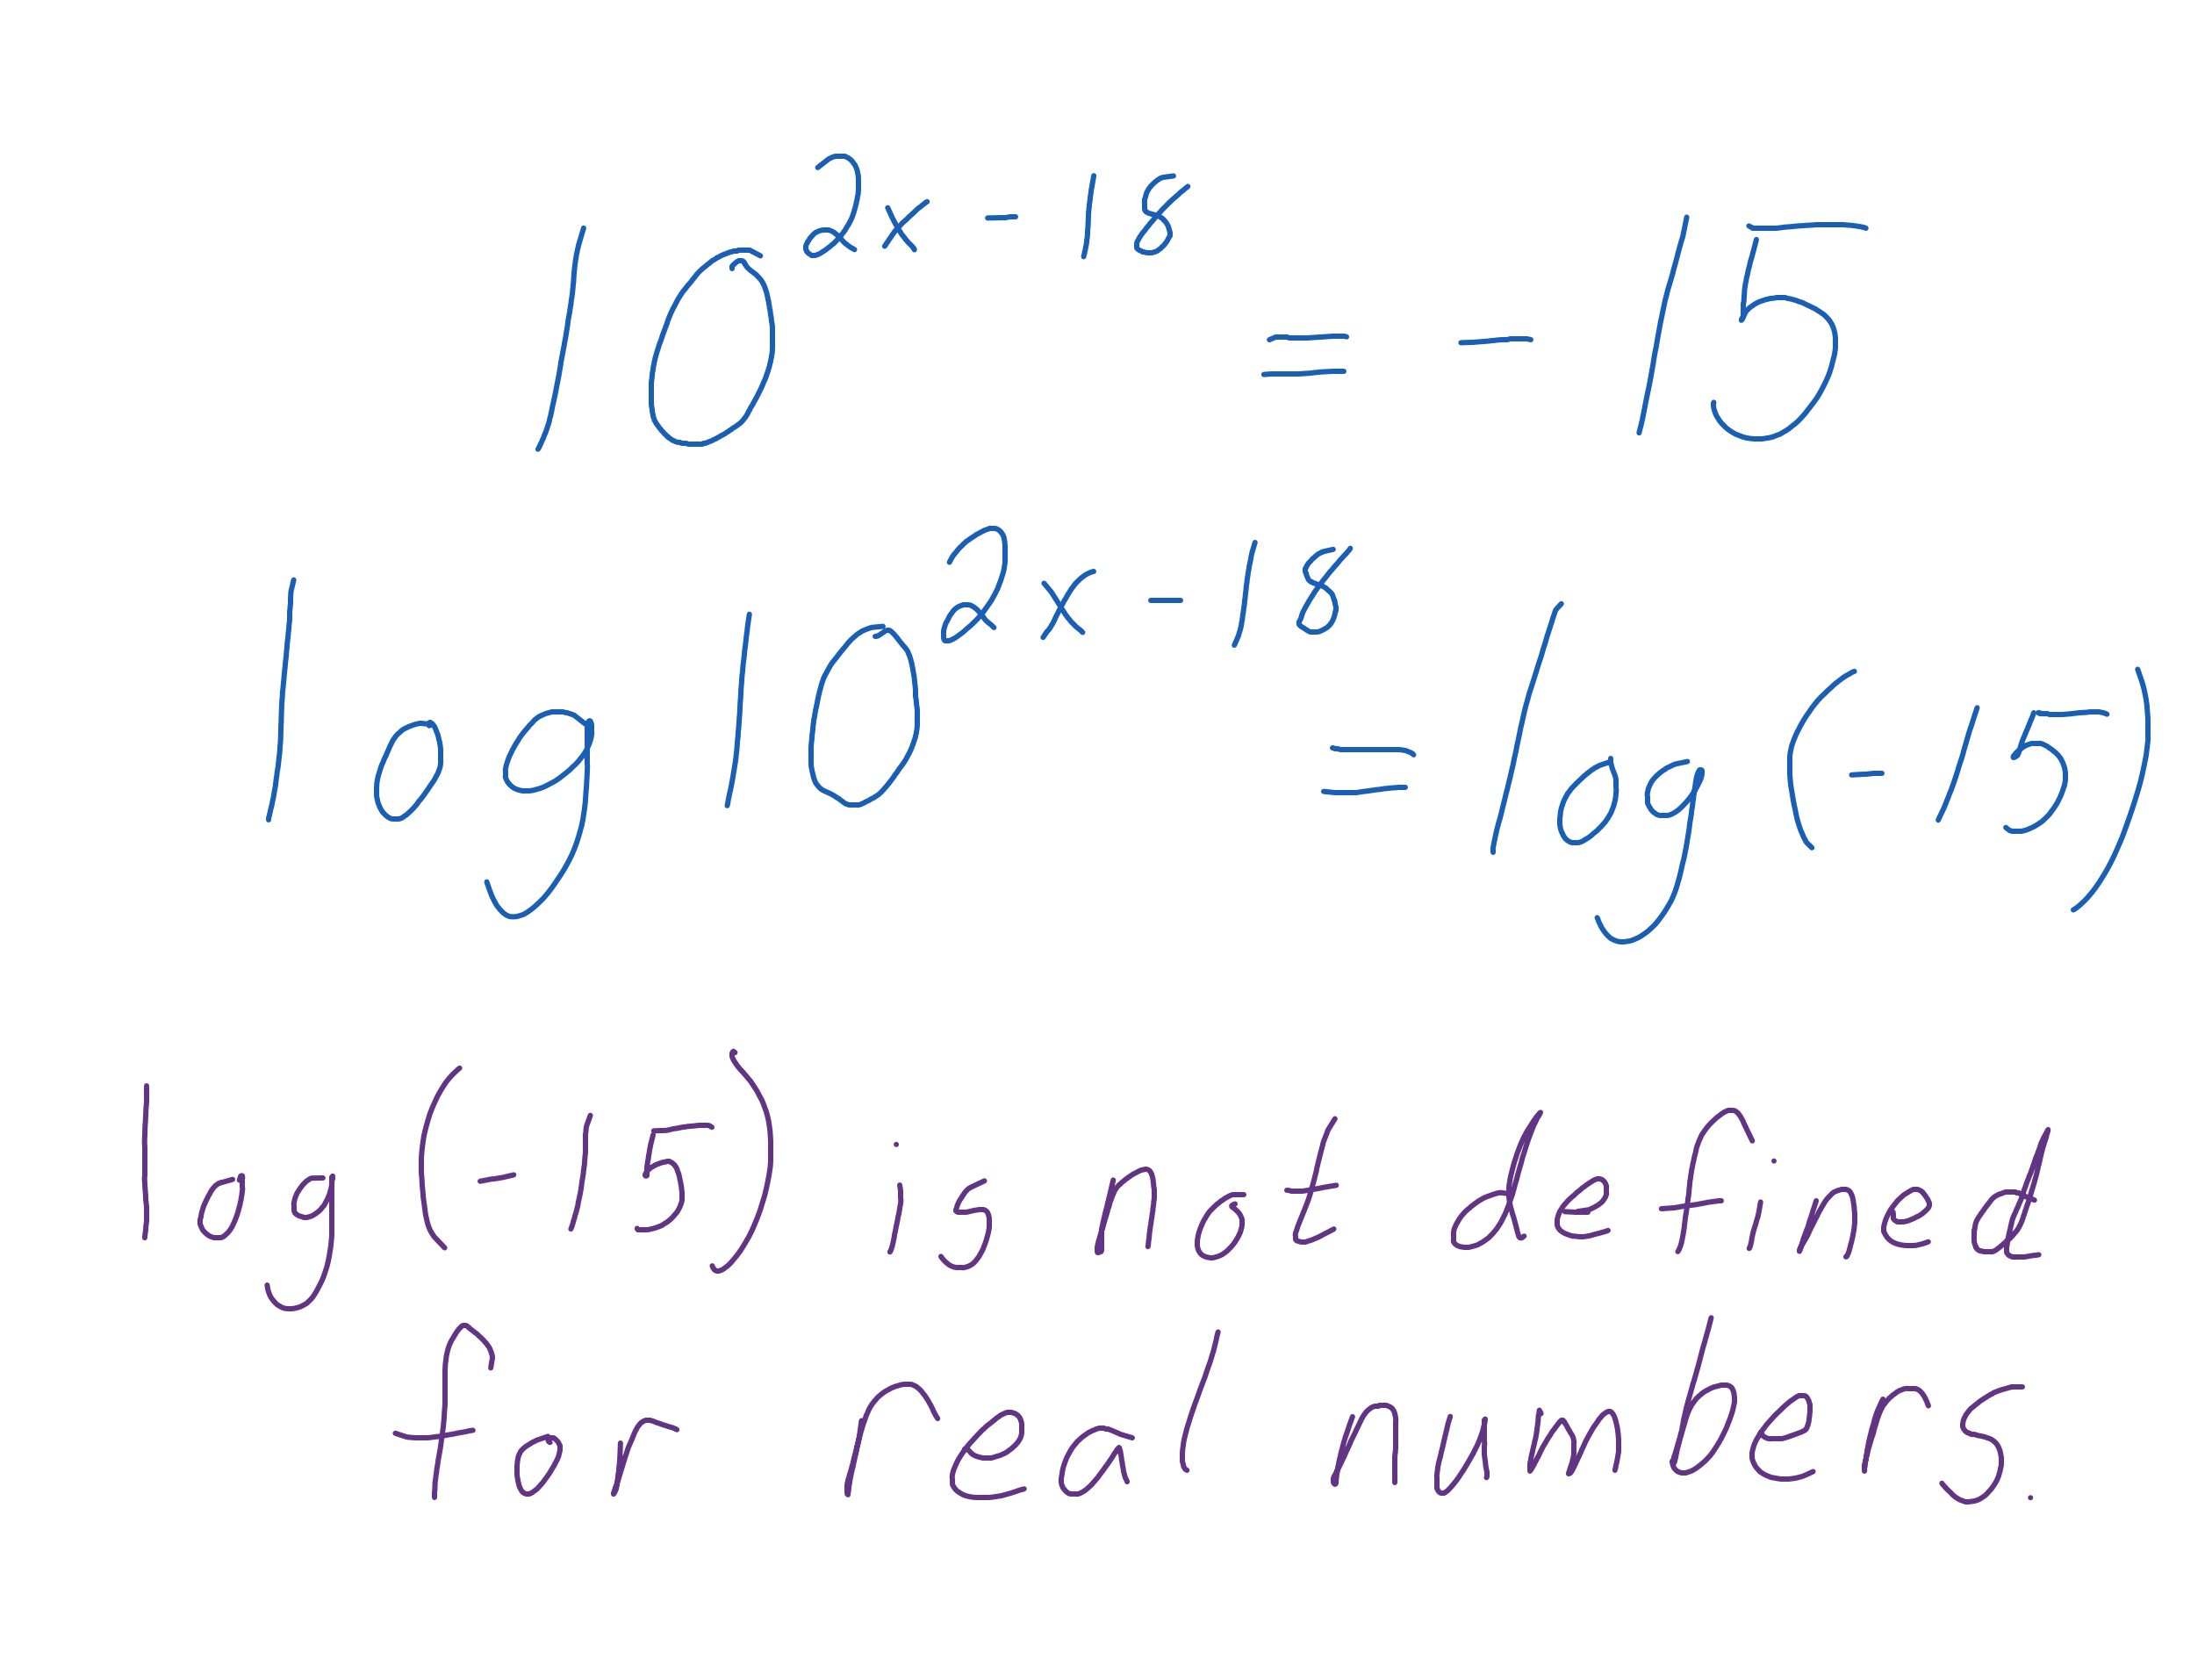
\includegraphics[width=\textwidth]{logarithmic_equations-work_05.png}
	\end{columns}
\end{frame}

\begin{frame}
	\frametitle{How To - Solve Logarithmic Equations}
	To solve an equation containing a logarithm: \pause
	\begin{enumerate}
		\item Isolate the logarithmic expression. \pause
		\item Use both sides as an exponent in an exponential expression. Use the same base for the exponential expression as the logarithm. \pause
		\item Cancel the exponential expression and logarithm using the Inverse Property. \pause
		\item Solve the resulting equation.
	\end{enumerate}
\end{frame}

\begin{frame}[t]
	\frametitle{Example 3}
	Solve the equation. Round your answer to three decimal places where appropriate.
	$$2 \cdot \log\left(6x\right) + 16 = 14$$
\end{frame}

\begin{frame}
	\frametitle{Example 3}
	\begin{columns}
		\column{0.3\textwidth}
			Solve for the logarithm.
		\column{0.7\textwidth}
			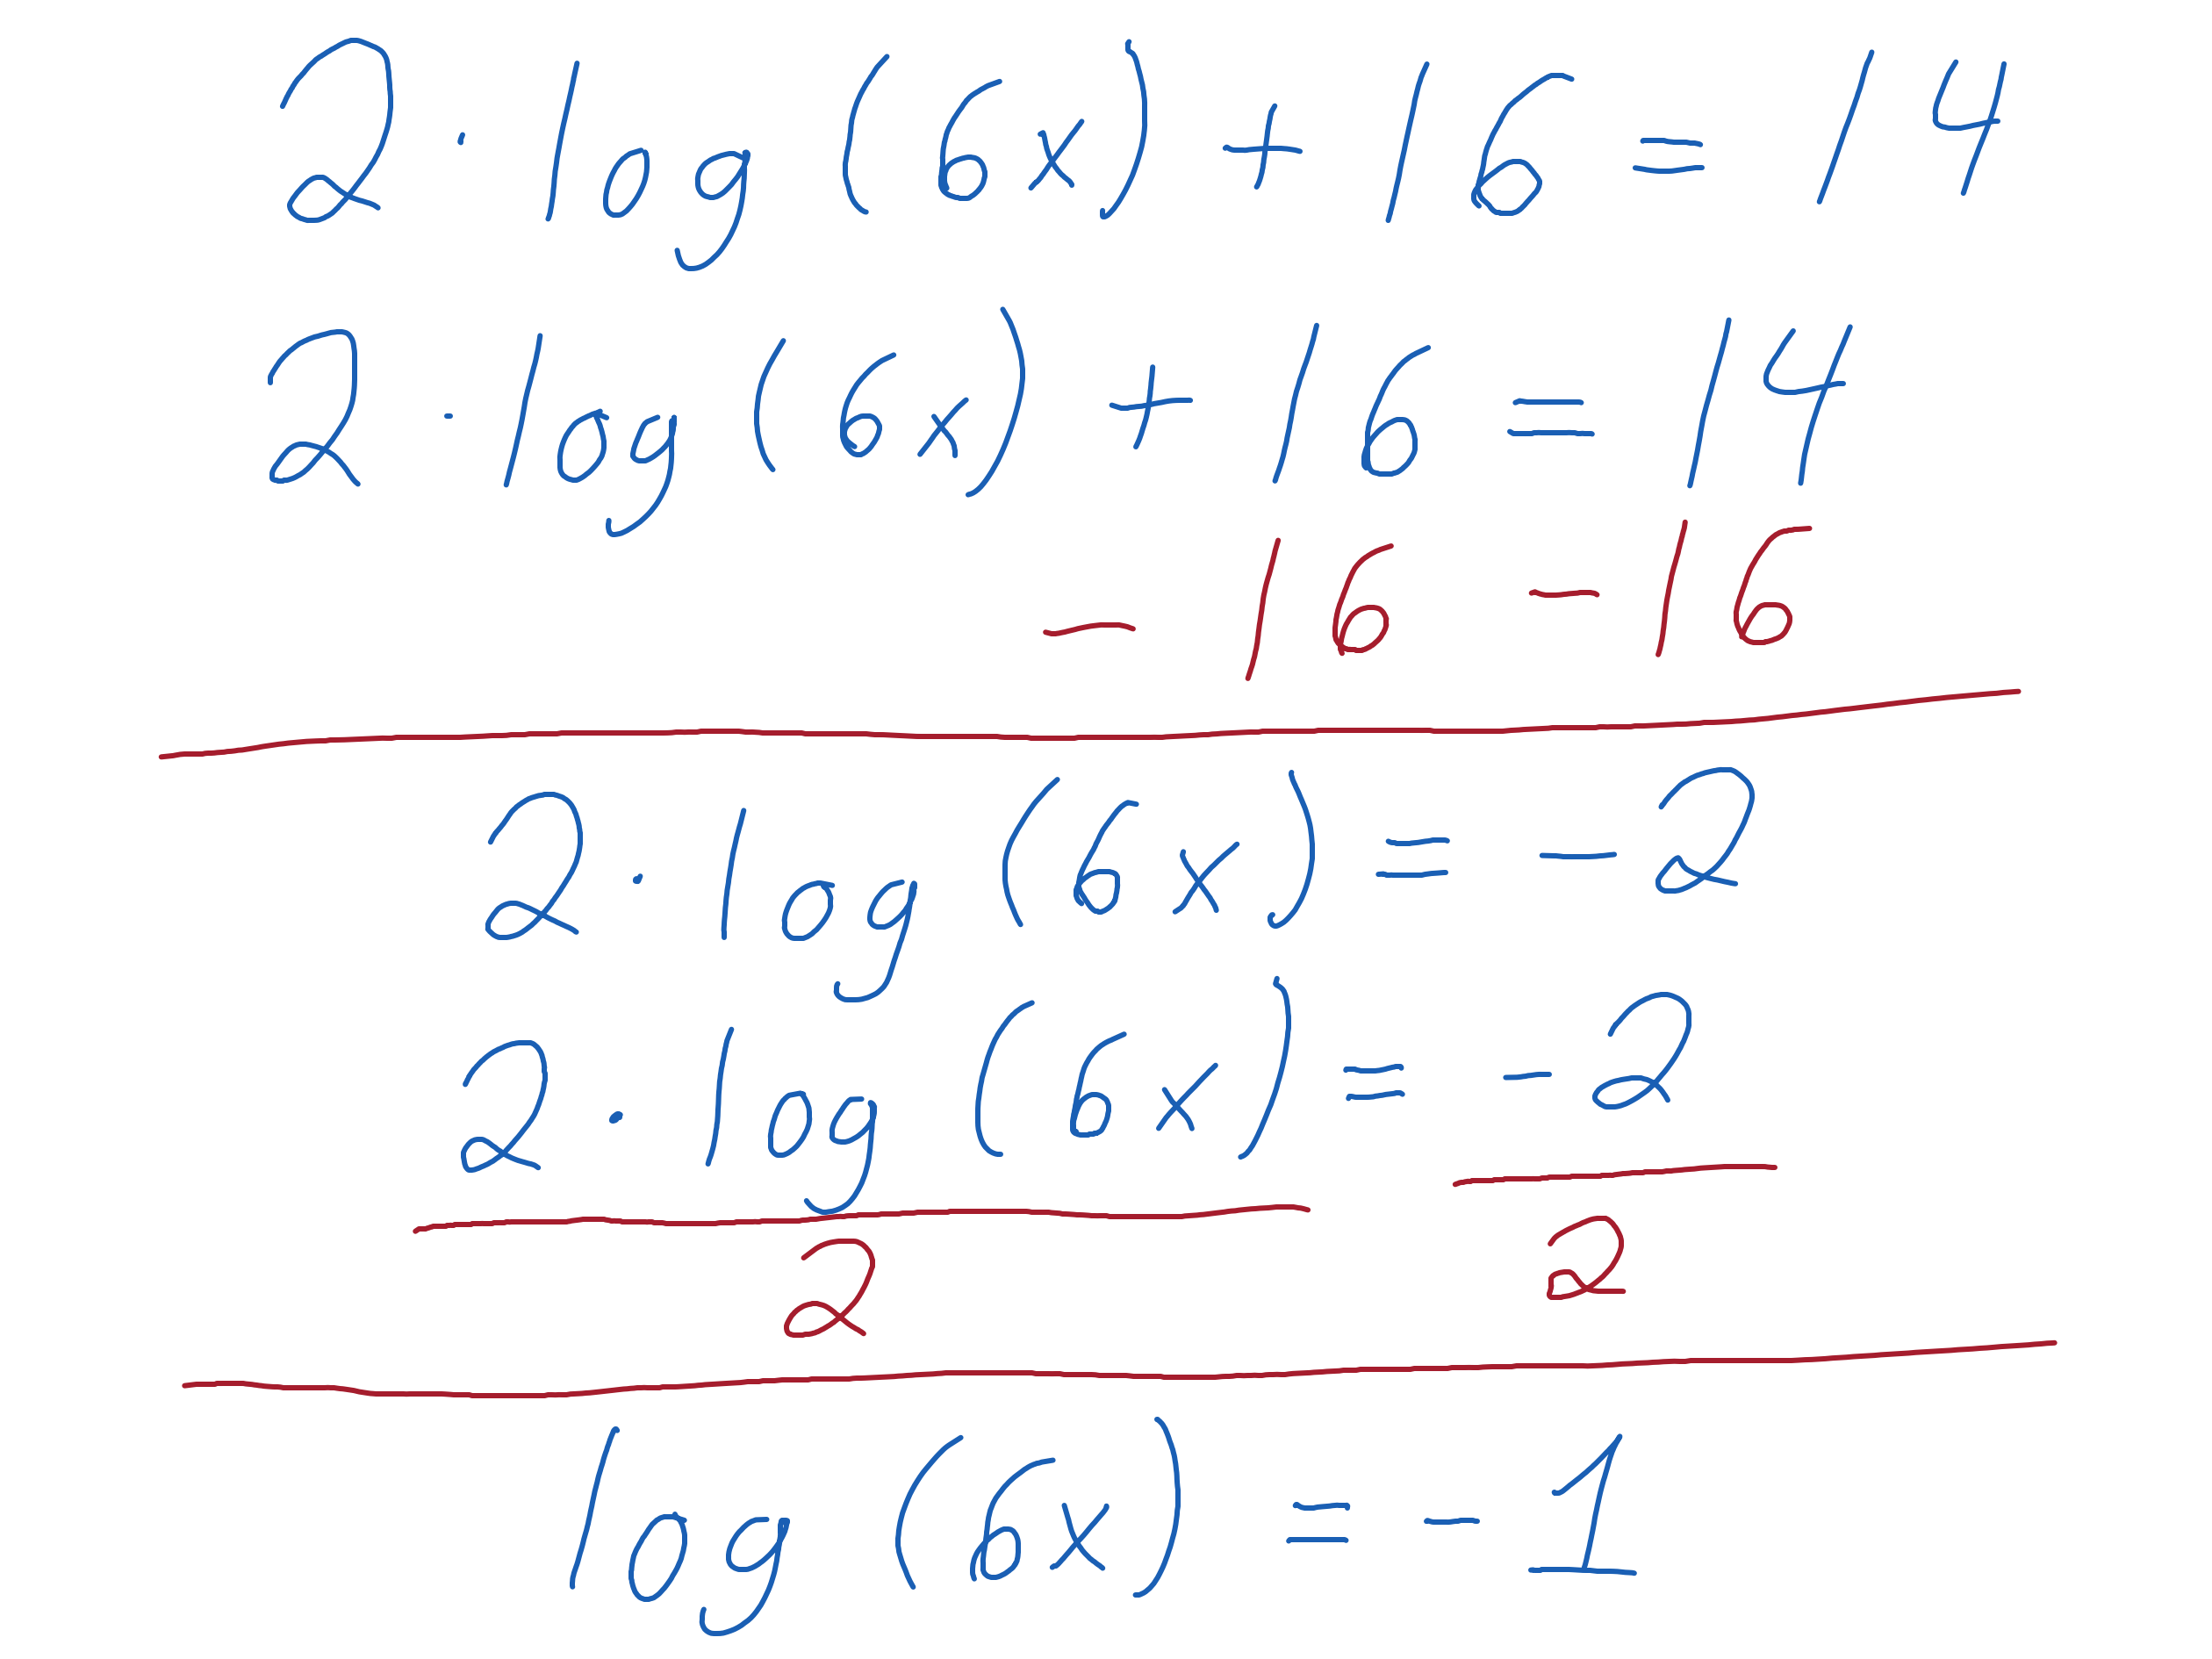
\includegraphics[width=\textwidth]{logarithmic_equations-work_06.png}
	\end{columns}
\end{frame}

\begin{frame}
	\frametitle{Example 3}
	\begin{columns}
		\column{0.3\textwidth}
		\begin{itemize} \small
			\item Use both sides as an exponent with base 10.
			\item Cancel the exponent and logarithm.
			\item The negative exponent is defined, so we know there are solutions.
		\end{itemize}
		\column{0.7\textwidth}
			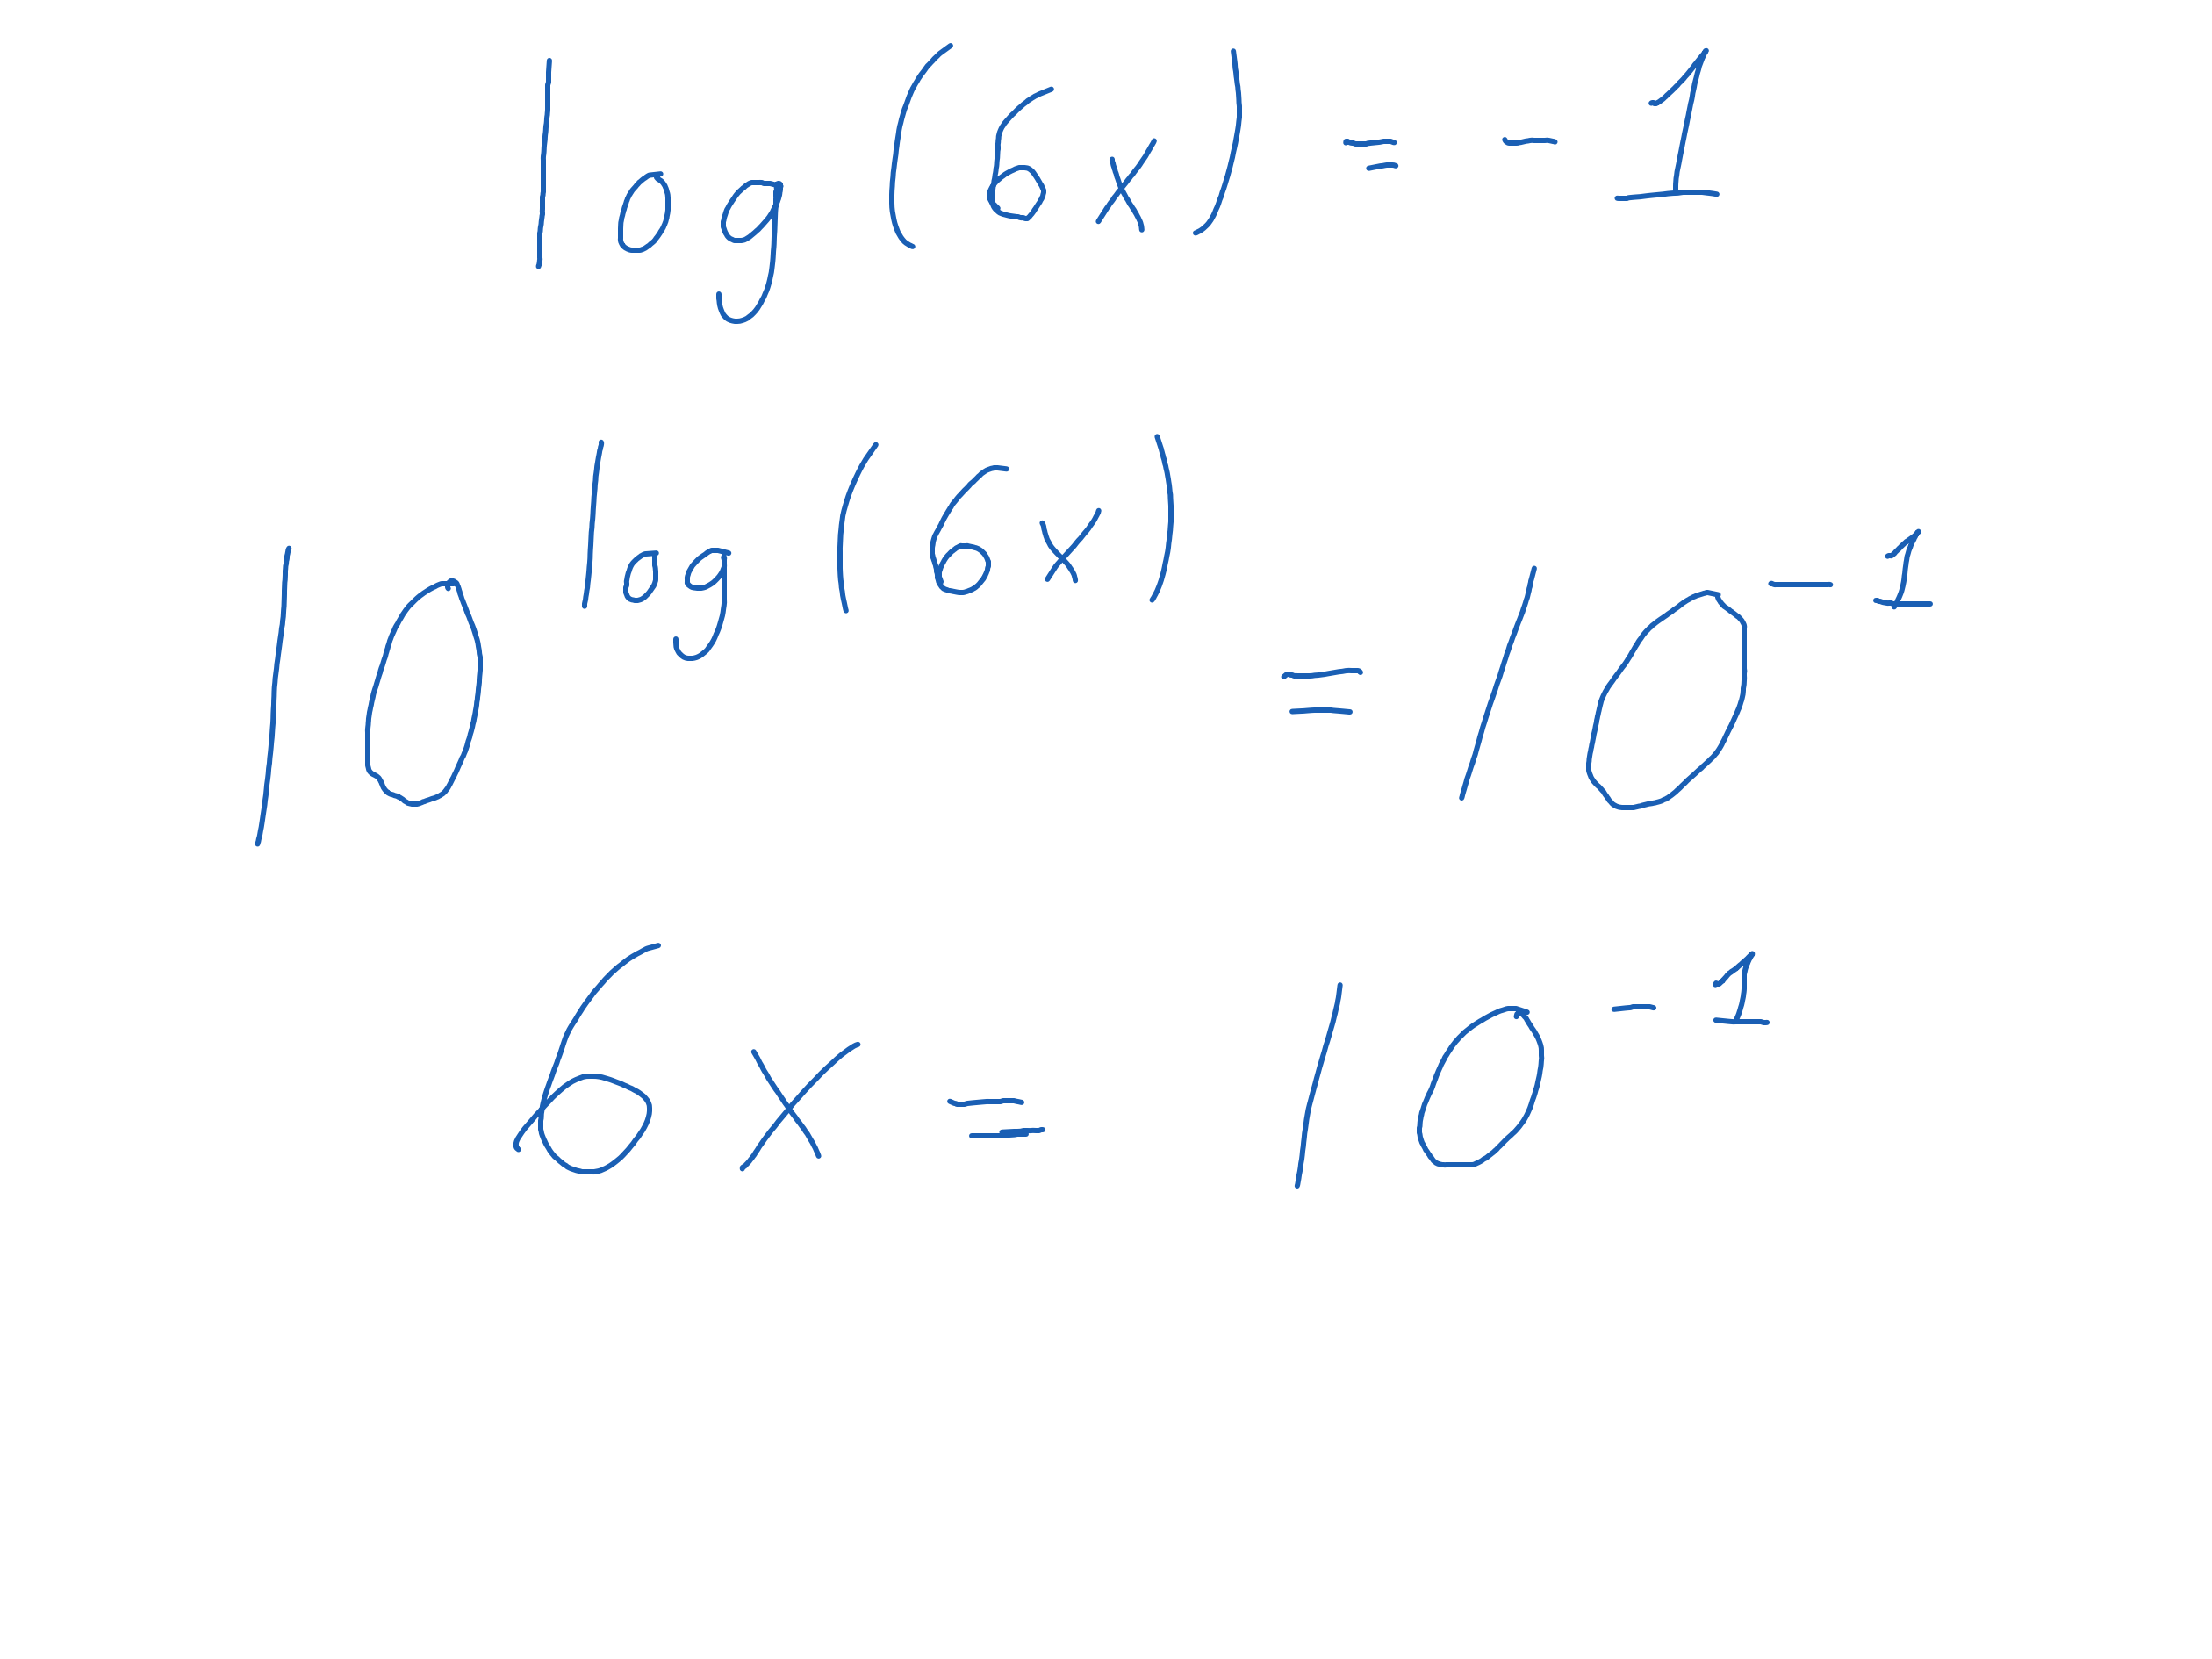
\includegraphics[width=\textwidth]{logarithmic_equations-work_07.png}
	\end{columns}
\end{frame}

\begin{frame}
	\frametitle{Example 3}
	\begin{columns}
		\column{0.3\textwidth}
		\begin{itemize} \small
			\item Solve the equation for $x$.
			\item Round the answer to three decimal places.
		\end{itemize}
		\column{0.7\textwidth}
			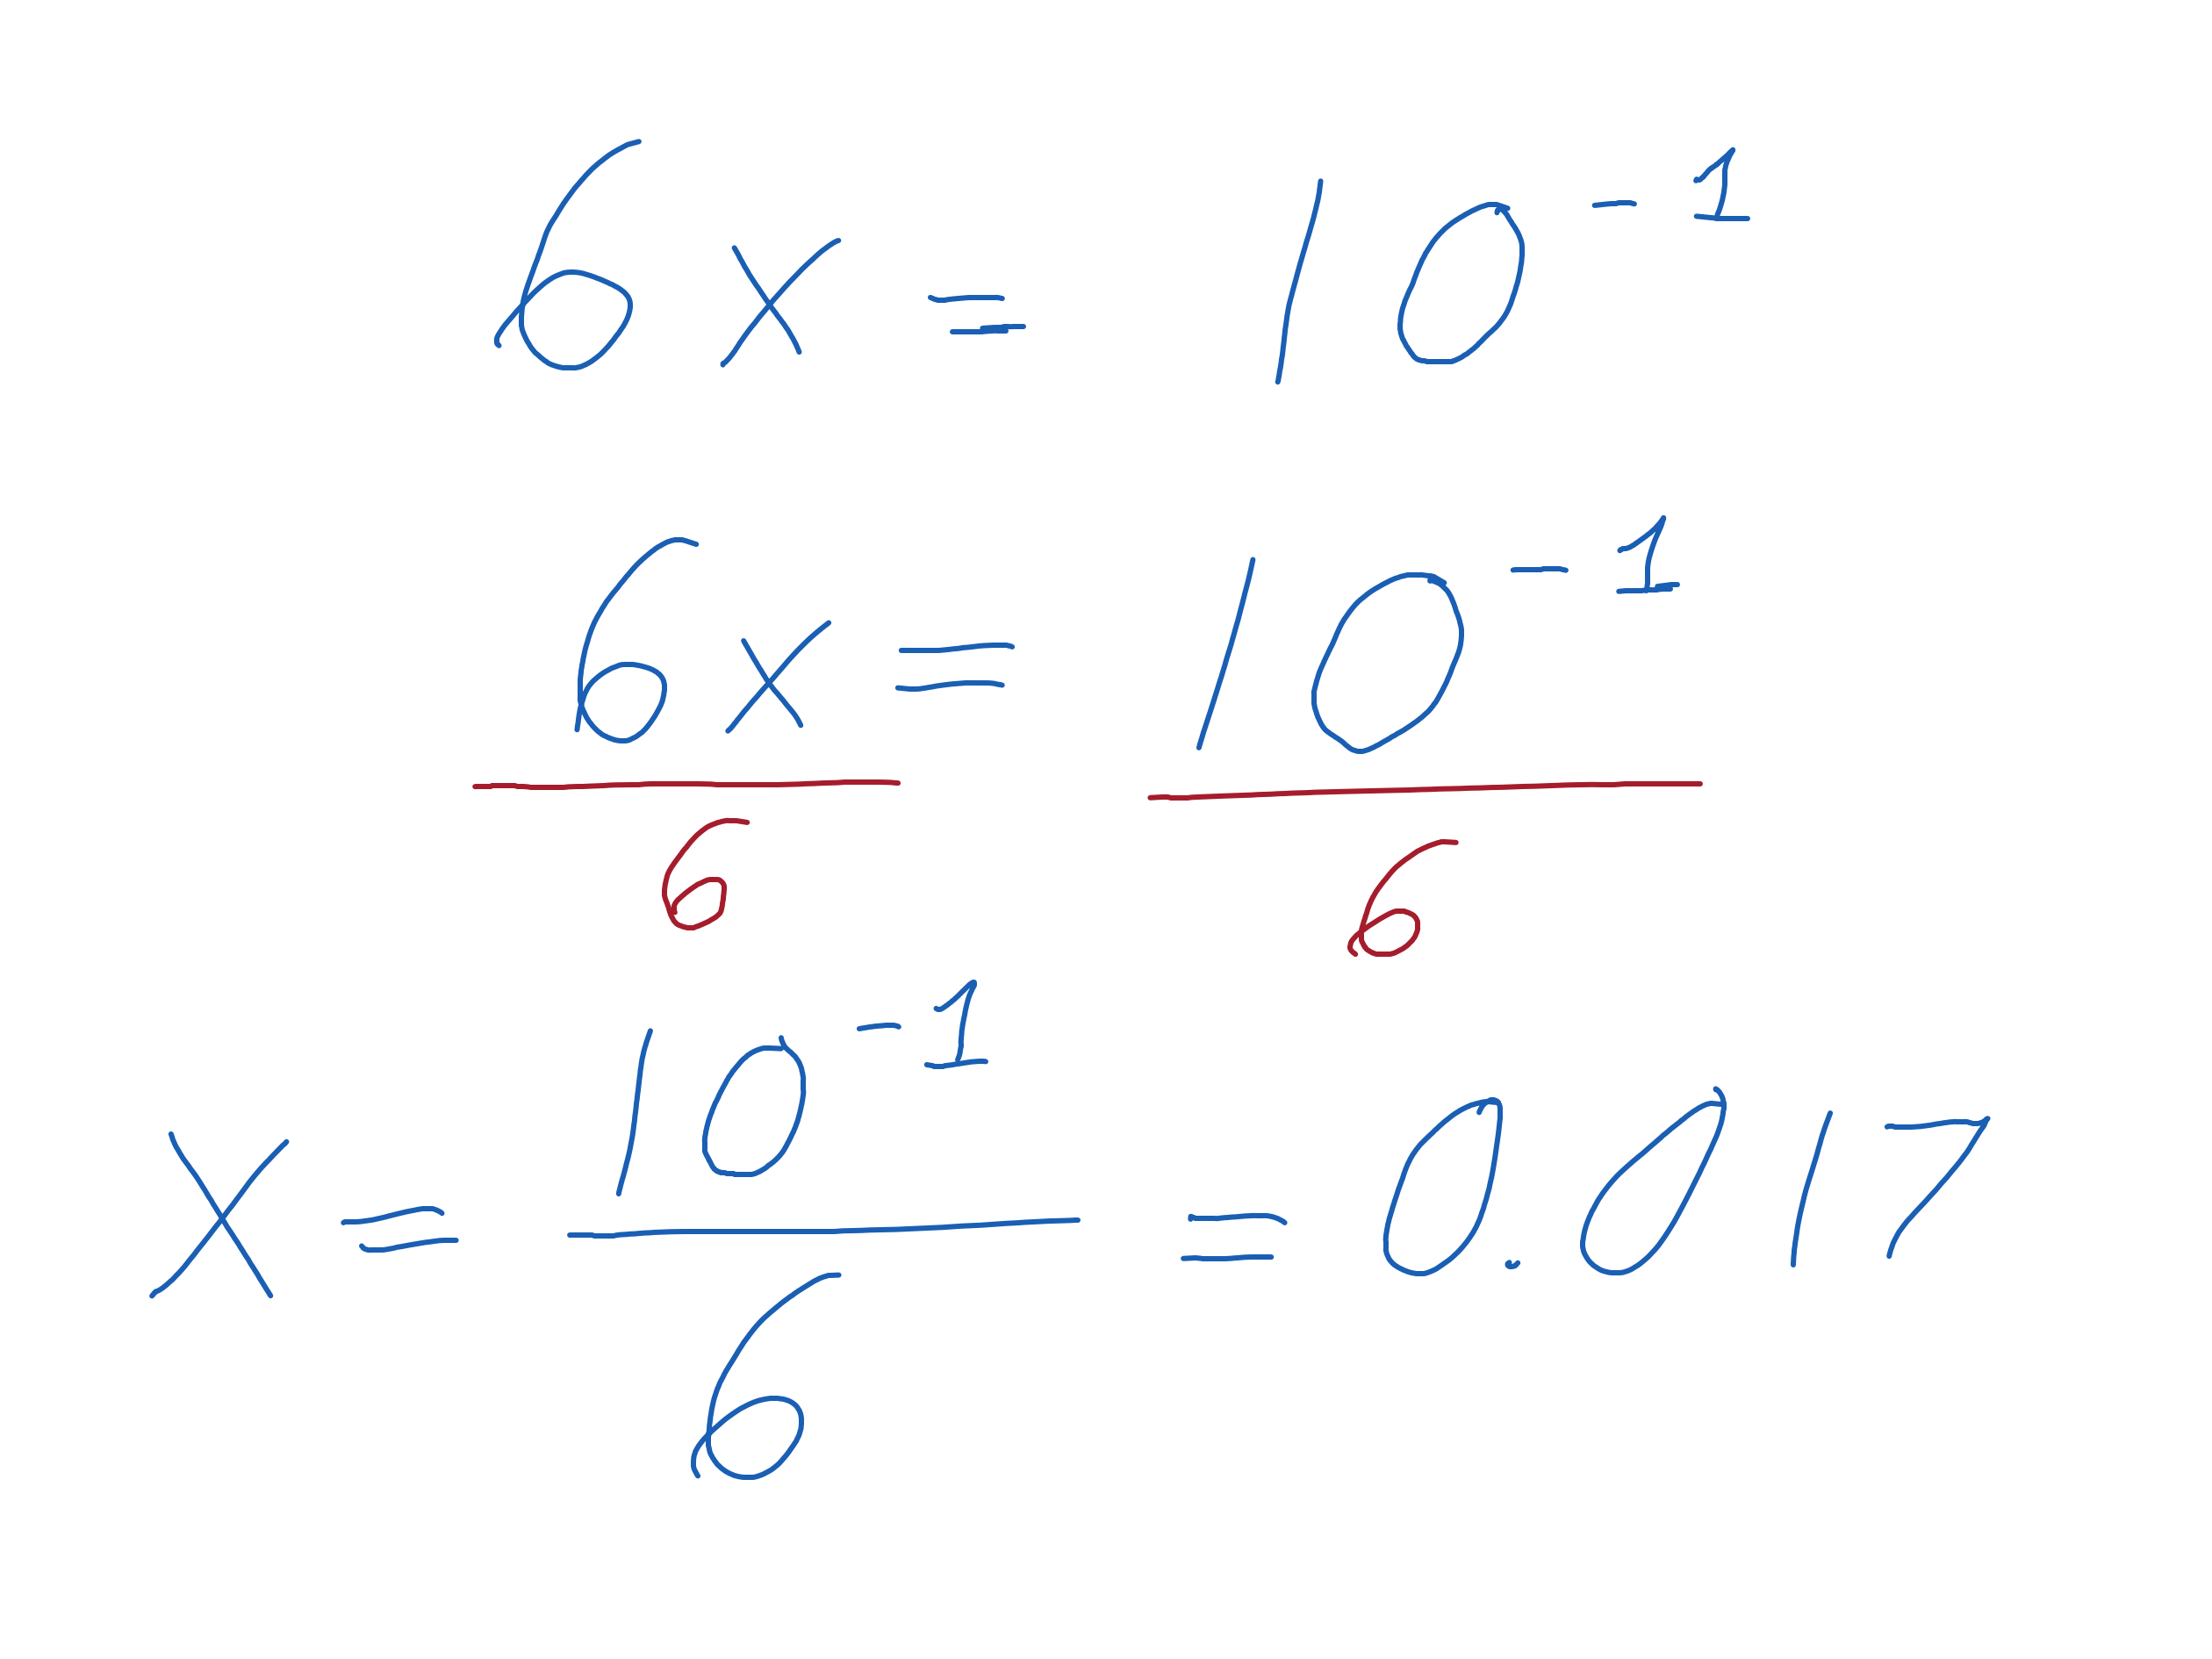
\includegraphics[width=\textwidth]{logarithmic_equations-work_08.png}
	\end{columns}
\end{frame}

\begin{frame}
	\frametitle{Example 3}
	\begin{columns}
		\column{0.3\textwidth}
		\begin{itemize} \small
			\item Solve the equation for $x$.
			\item Round the answer to three decimal places.
		\end{itemize}
\column{0.7\textwidth}
			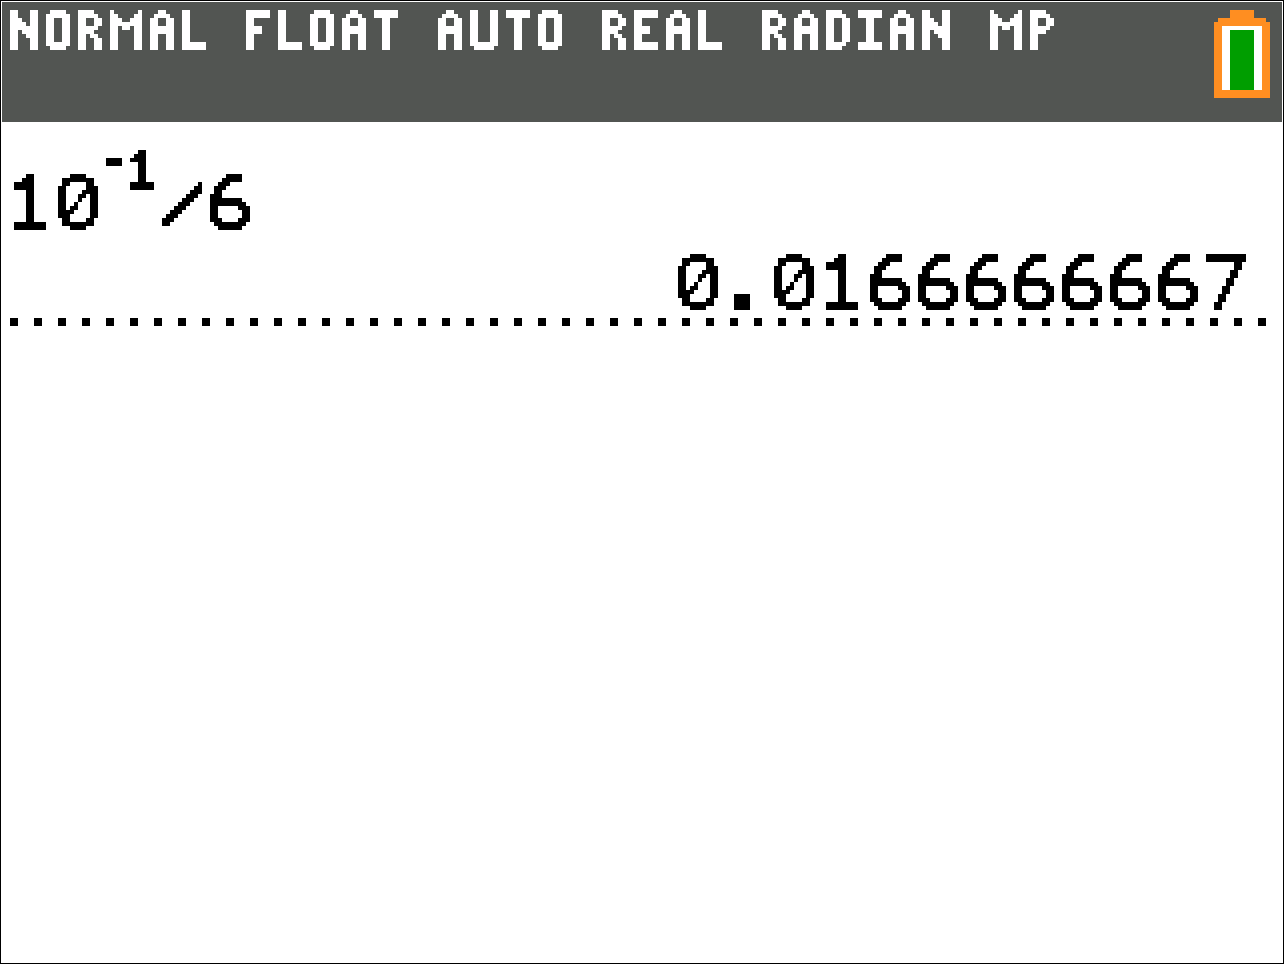
\includegraphics[width=\textwidth]{Capture 2.png}
	\end{columns}
\end{frame}

\begin{frame}[t]
	\frametitle{Example 4}
	Solve the equation. Round your answer to three decimal places where appropriate.
	$$\log_8{\left(3x-18\right)} = 3$$
\end{frame}

\begin{frame}
	\frametitle{Example 4}
	\begin{columns}
		\column{0.3\textwidth}
		\begin{itemize}\small
			\item Use both sides of the equation as an exponent with base $8$.
			\item Cancel the exponent and logarithm.
		\end{itemize}
		\column{0.7\textwidth}
			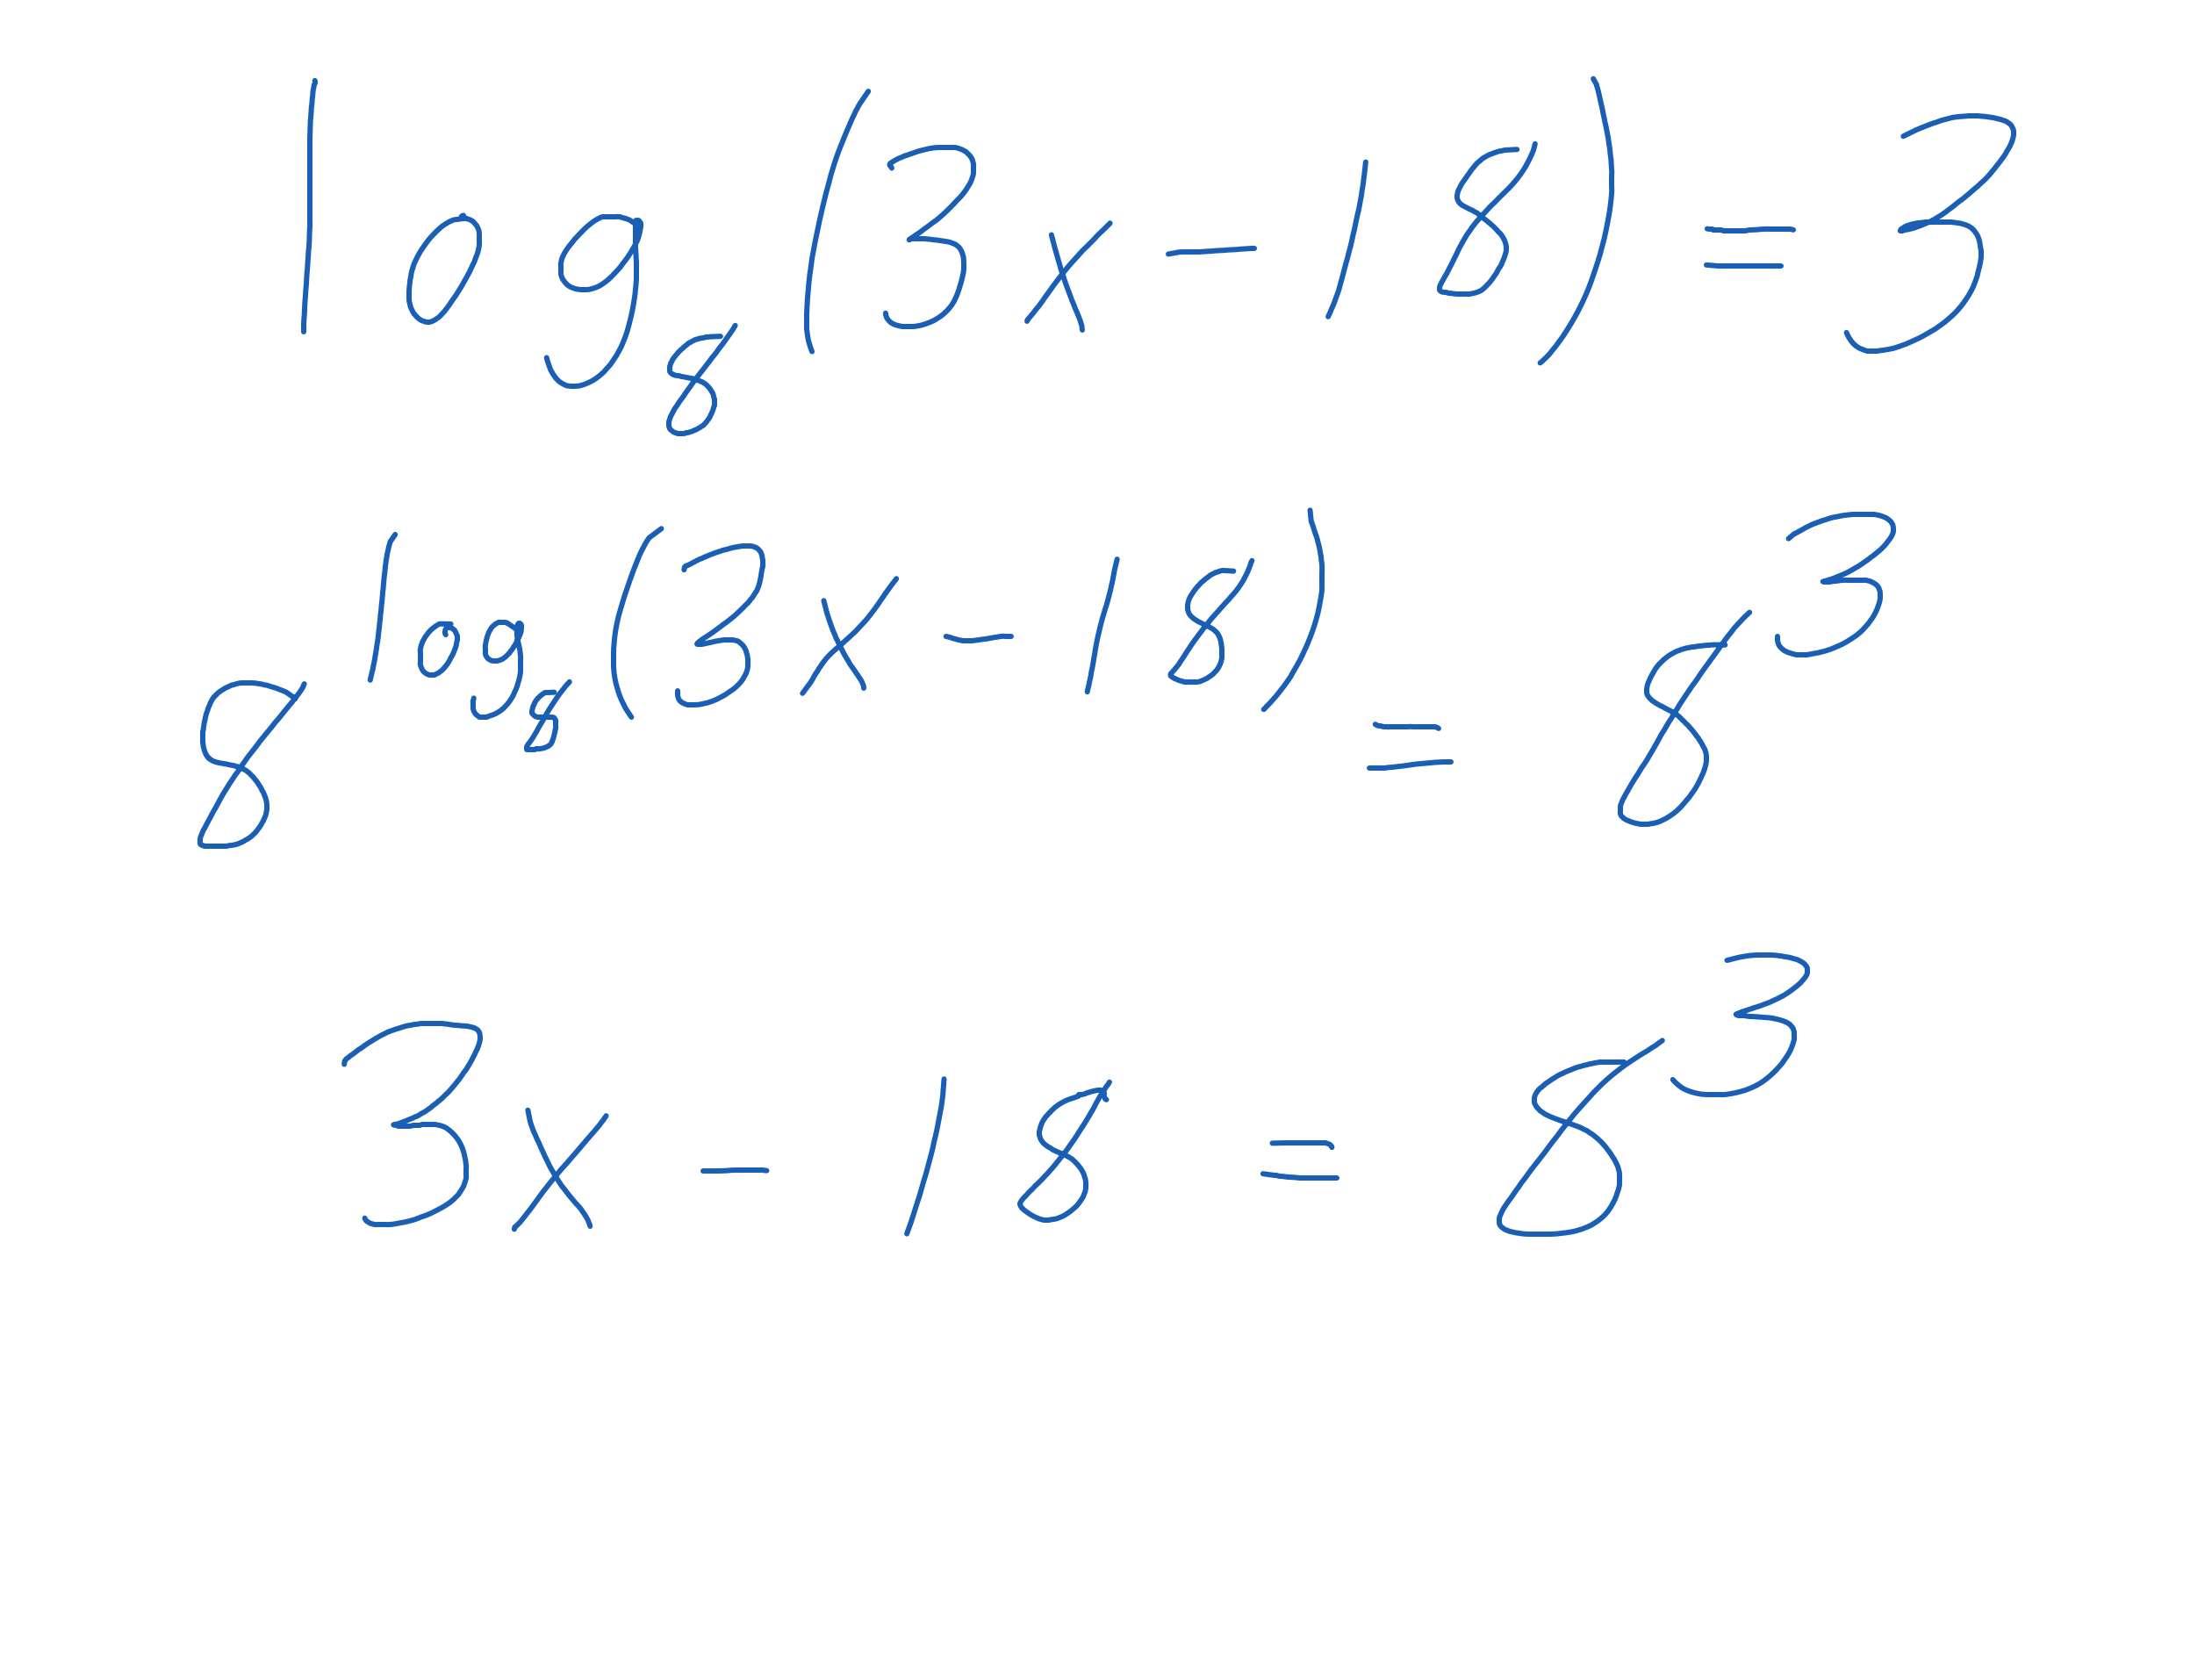
\includegraphics[width=\textwidth]{logarithmic_equations-work_09.png}
	\end{columns}
\end{frame}

\begin{frame}
	\frametitle{Example 4}
	\begin{columns}
		\column{0.3\textwidth}
		\begin{itemize} \small
			\item Solve the equation for $x$.
			\item Round the answer to three decimal places.
		\end{itemize}
		\column{0.7\textwidth}
			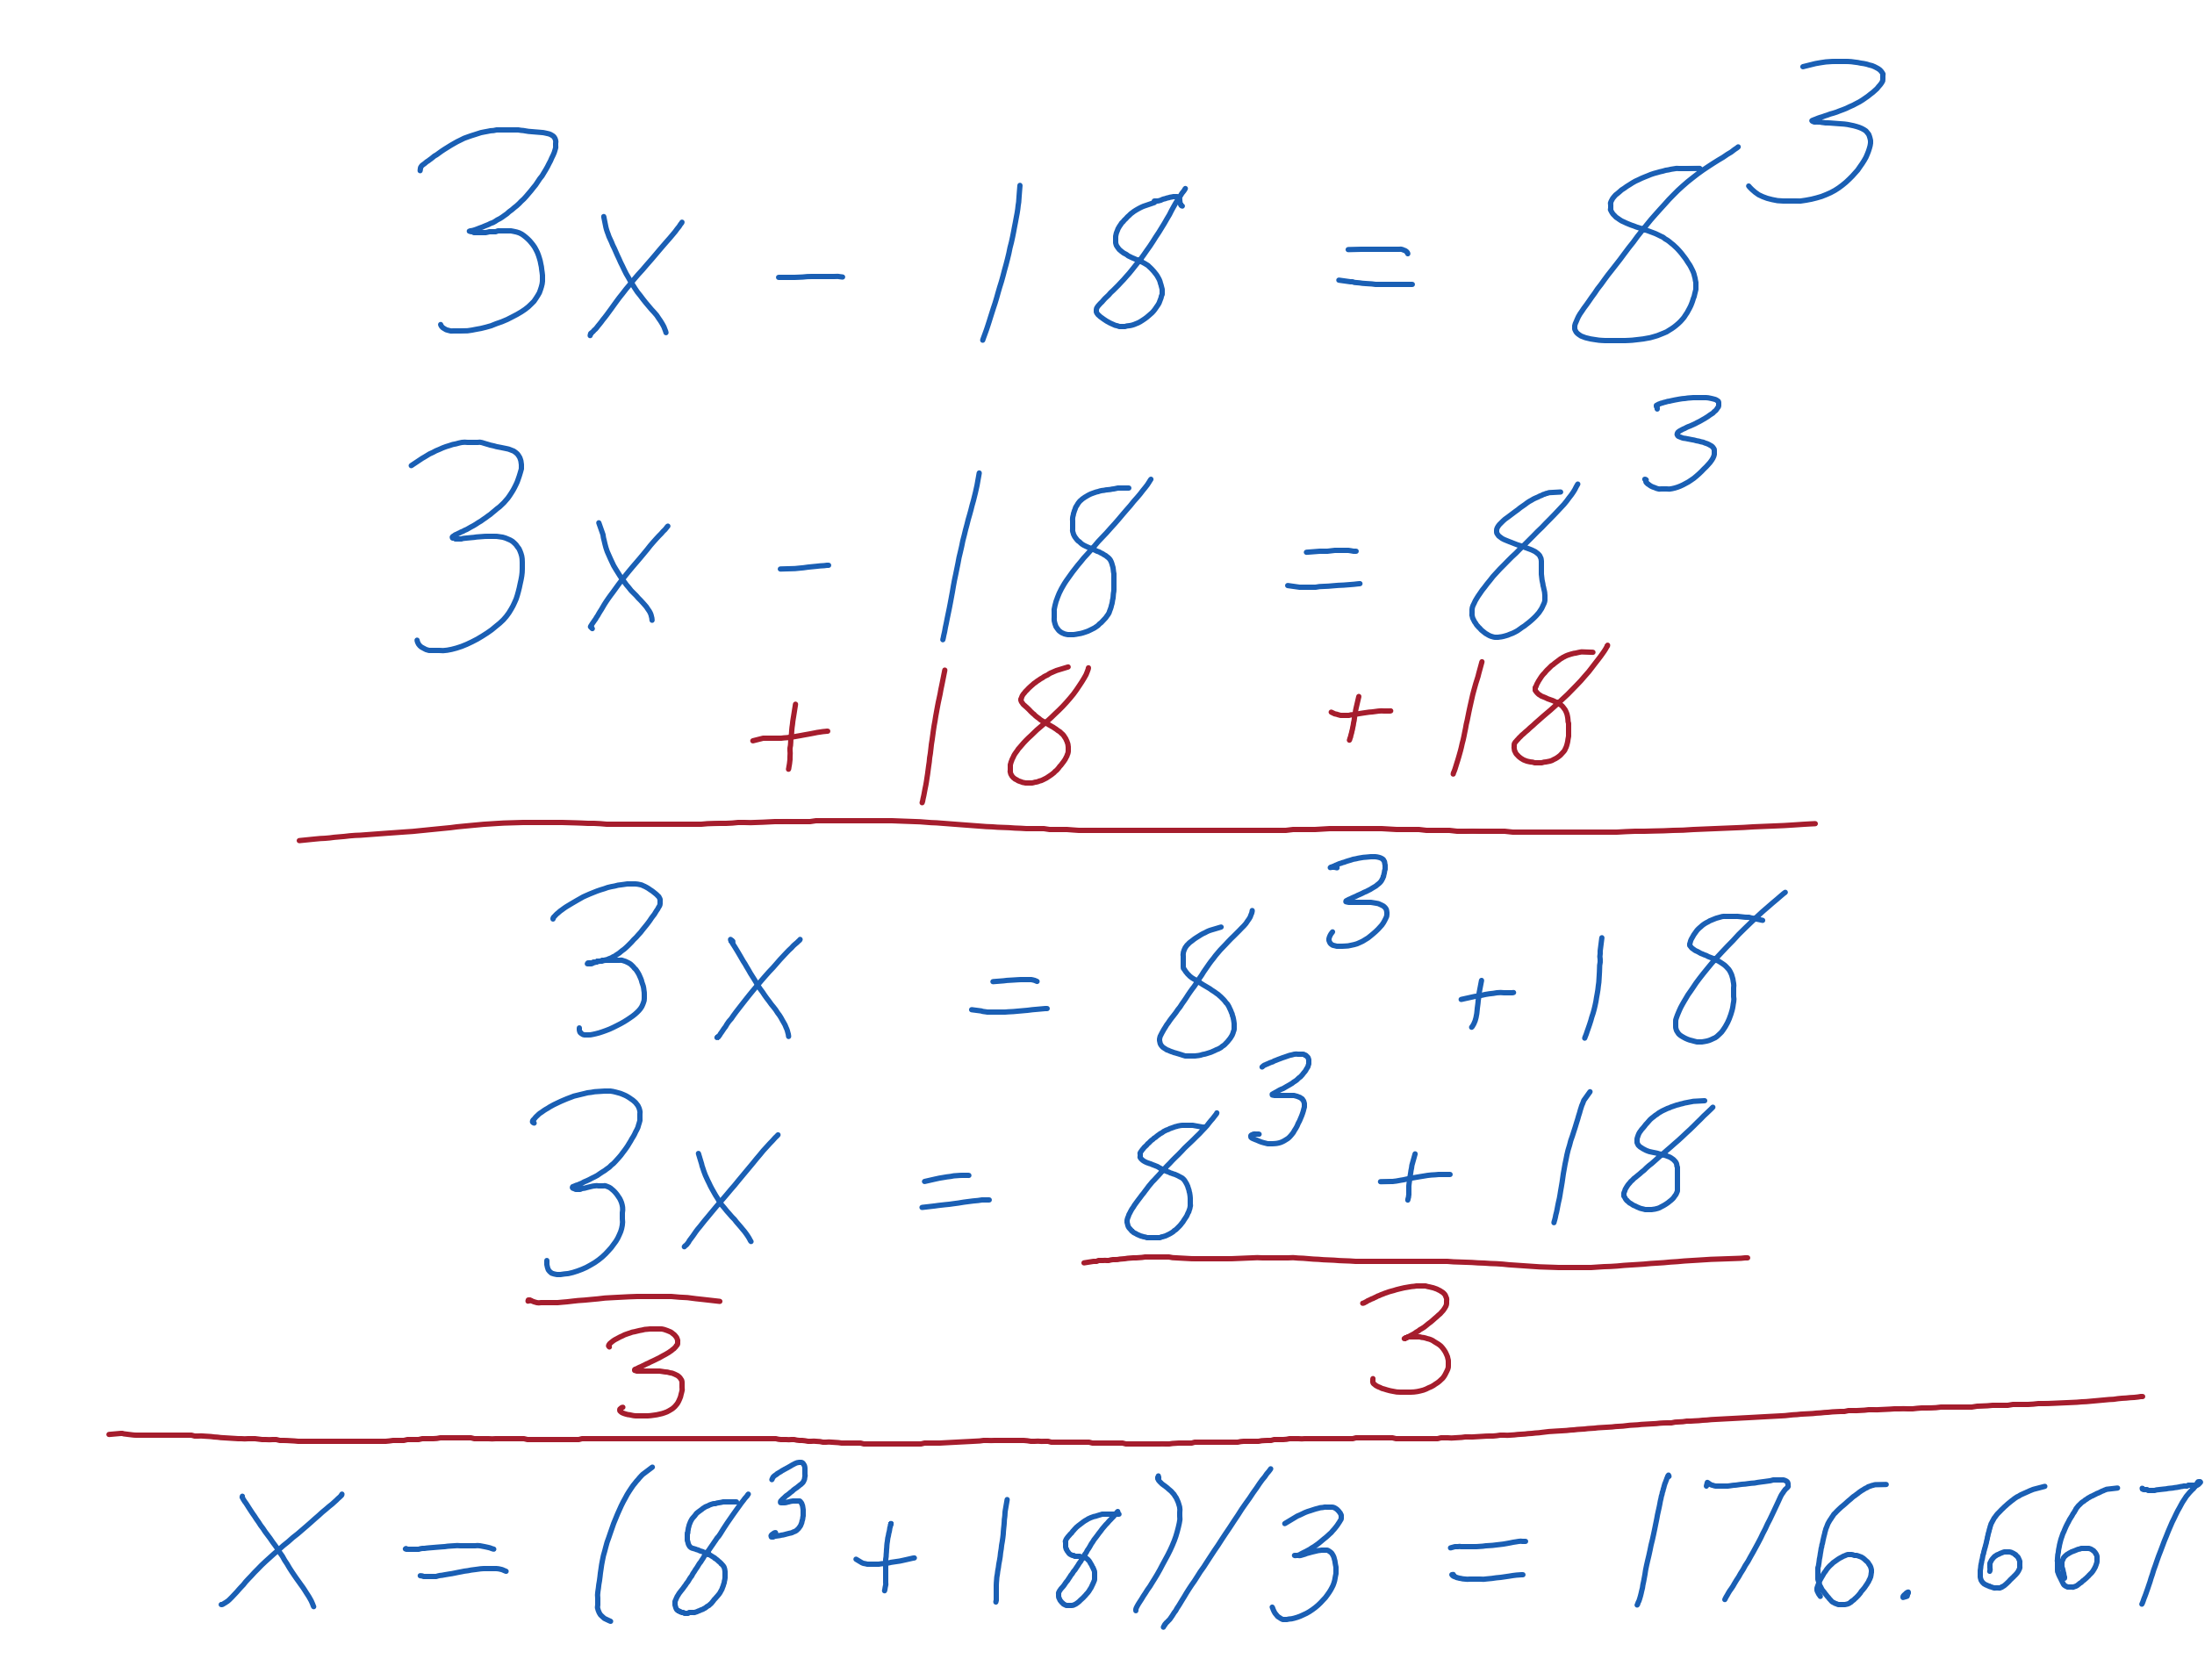
\includegraphics[width=\textwidth]{logarithmic_equations-work_10.png}
	\end{columns}
\end{frame}

\begin{frame}
	\frametitle{Example 4}
	\begin{columns}
		\column{0.3\textwidth}
		\begin{itemize} \small
			\item Solve the equation for $x$.
			\item Round the answer to three decimal places.
		\end{itemize}
		\column{0.7\textwidth}
			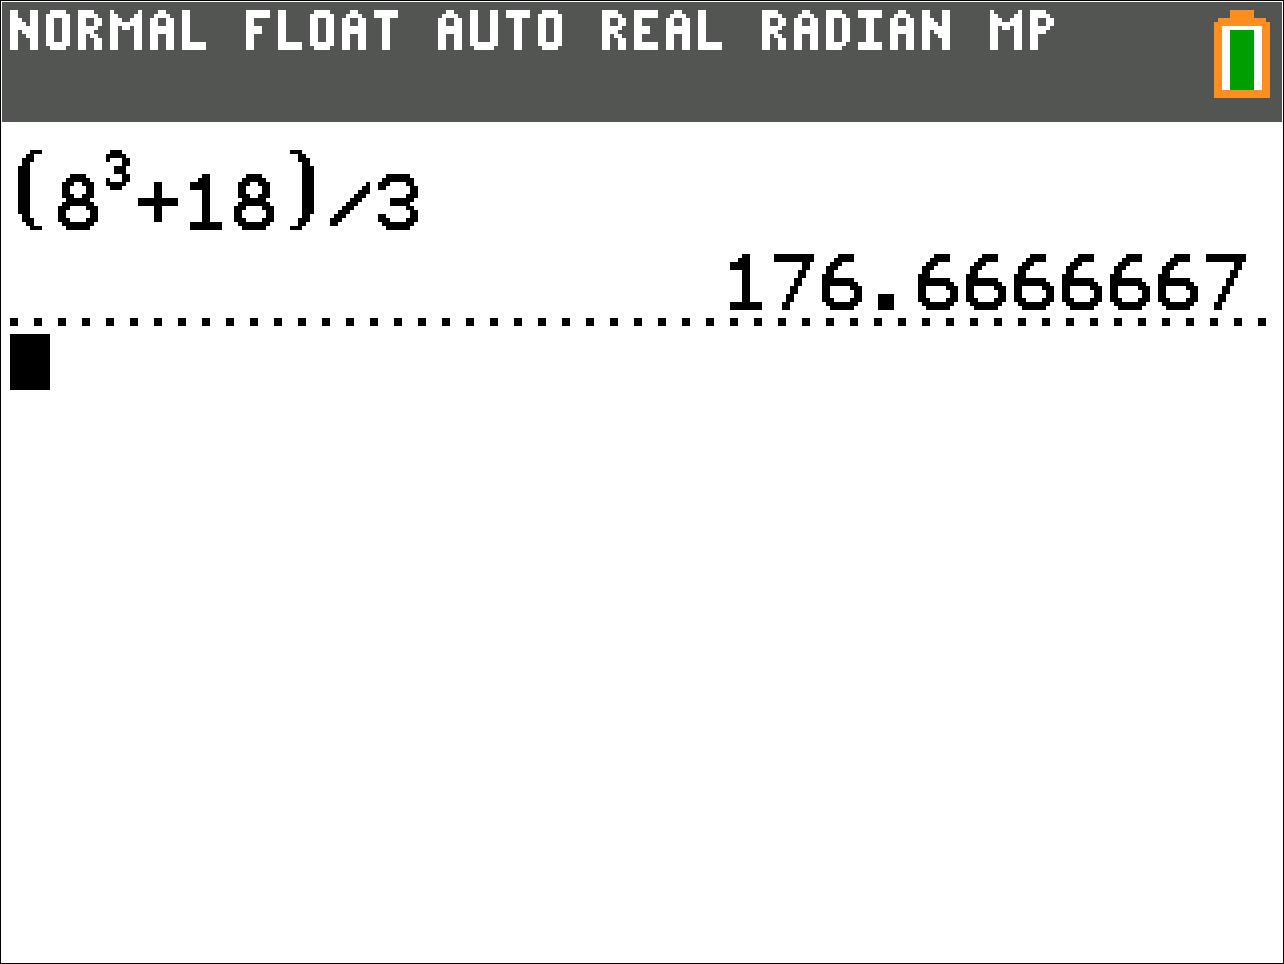
\includegraphics[width=\textwidth]{Capture 3.png}
	\end{columns}
\end{frame}

\end{document}